%********************************************************************
% Appendix
%*******************************************************
% If problems with the headers: get headings in appendix etc. right
%\markboth{\spacedlowsmallcaps{Appendix}}{\spacedlowsmallcaps{Appendix}}
\chapter{Calculation Details to Chapter 2}
\section{Kubo formula}
The linear response formula used in the main text can be obtained in a Keldysh-framework. We start by introducing the Green function $\mathcal{G}$ in rotated Keldysh space [see e.g. Ref.~\cite{rammer_quantum_1986}]
\begin{equation}
    \mathcal{G}=\begin{pmatrix}G^\text{R}&G^\text{K}\\0&G^\text{A}\end{pmatrix}
\end{equation}
where R, A and K denote retarded, advanced and Keldysh Green functions respectively. In this notation a perturbation to a classical field $V(\bb{x},t)$ is given by
\begin{multline}
    \delta\mathcal{G}(\bb{x}_1,t_1;\bb{x}_2,t_2)=\int\!d\bb{x}_3\int\!dt_3\, \mathcal{G}^{(0)}(\bb{x}_1,t_1;\bb{x}_3,t_3)\\\hat{V}(\bb{x}_3,t_3)\mathcal{G}^{(0)}(\bb{x}_3,t_3;\bb{x}_2,t_2)+\mathcal{O}(V^2)
    \label{chap1:eq:s2}
\end{multline}
with $\mathcal{G}^{(0)}$ equilibrium Green functions. The Wigner-transform of a function $F(\bb{x}_1,t_1;\bb{x}_2,t_2)$ is given by
  \begin{multline}
    F(\bb{x}_1,t_1;\bb{x}_2,t_2)=\int\frac{d^2\bb{p}}{(2\pi\hslash)^2}\int \frac{d\ep}{2\pi\hslash}\,e^{-i\ep(t_1-t_2)/\hslash}e^{i\bb{p}\cdot(\bb{x}_1-\bb{x}_2)/\hslash}F(\ep,\bb{p},R,T)
   \end{multline}
with energy $\ep$, momentum $\bb{p}$, time $T=\frac{t_1+t_2}{2}$ and position $\bb{R}=\frac{\bb{x}_1+\bb{x}_2}{2}$. In equilibrium the Green functions $\mathcal{G}^{(0)}$ do not depend on $\bb{R}$ and $T$, so that the momentum-frequency representation of Eq.~(\ref{chap1:eq:s2}) becomes 
   $\delta\mathcal{G}(\ep,\omega,\bb{p},\bb{q})= \mathcal{G}^{(0)}_{\ep_+,\bb{p}_+} V_{\omega,\bb{q}}\mathcal{G}^{{(0)}}_{\ep_-,\bb{q}_-}$, 
with subscripts $\ep_\pm=\ep\pm\hslash\omega/2$ and $\bb{p}_\pm=\bb{p}\pm\hslash\bb{q}/2$ and $V_{\omega,\bb{q}}$ the Fourier transform of $V(\bb{R},T)$. 

The spin density $\bb{s}_{\omega,\bb{q}}$ is given by
\begin{equation}
    \bb{s}_{\omega,\bb{q}} = {i\hslash} \int\!\frac{d\ep}{2\pi\hslash}\int\!\frac{d^2\bb{p}}{(2\pi\hslash)^2}\tr \left[\delta G^<({\ep,\omega,\bb{p},\bb{q}},T) \bb{\sigma}\right],
\end{equation}
where,
\begin{multline}
    \delta G^<(\ep,\omega,\bb{p},\bb{q}) = 1/2 \big(\delta G^\text{K}(\ep,\omega,\bb{p},\bb{q})-
    \delta G^\text{R}(\ep,\omega,\bb{p},\bb{q})+\delta G^\text{A}(\ep,\omega,\bb{p},\bb{q})\big).  
\end{multline}
In equilibrium we have the fluctuation-dissipation theorem $   G^\text{K}_{\ep_\pm,\bb{p}_\pm} = (1-2f_{\ep_\pm})(G^\text{R}_{\ep_\pm,\bb{p}_\pm}-G^\text{A}_{\ep_\pm,\bb{p}_\pm}) $ with $f_{\ep_\pm}$ the Fermi distribution, so that the spin density now becomes
\begin{align}
    \bb{s}_{\omega,\bb{q}} = {i\hslash} \int\!\frac{d\ep}{2\pi\hslash}\int\!\frac{d^2\bb{p}}{(2\pi\hslash)^2}\tr\langle\nonumber
     -(f_{\ep_+}-f_{\ep_-})\bb{\sigma}G^\text{R}_{\ep_+,\bb{p}_+} V_{\omega,\bb{q}}G^\text{A}_{\ep_-,\bb{p}_-}\nonumber
    -f_{\ep_+}\bb{\sigma}G^\text{R}_{\ep_+,\bb{p}_+} V_{\omega,\bb{q}}G^\text{R}_{\ep_-,\bb{p}_-}\nonumber
    +f_{\ep_-}\bb{\sigma}G^\text{A}_{\ep_+,\bb{p}_+} V_{\omega,\bb{q}}G^\text{A}_{\ep_-,\bb{p}_-}\rangle,
\end{align}
where the angular brackets stands for impurity averaging. The latter amounts to the replacement of the Green's functions with the corresponding impurity averaged Greens functions (in Born approximation) and to the replacement of one of the spin operators with the corresponding vertex corrected operator (in the non-crossing approximation). The corrections beyond the non-crossing approximation are important for those tensor components that lack leading-order contribution \cite{ivan}. To keep our notations more compact we ignore here the fact that the Green's functions before disorder averaging lack translational invariance, i.\,e. depend on both Wigner coordinates: momentum and coordinate. 

In the limit of small frequency, i.e. $\hslash\omega\ll\ep$, we obtain $s_\alpha = s^\text{I}_\alpha+s^\text{II}_\alpha$,
\begin{align}
    s^\text{I}_\alpha&=\frac{i\omega}{2\hslash}\int\frac{d\ep}{2\pi}\int \frac{d^2\bb{p}}{(2\pi)^2}\Big(-\frac{\partial f}{\partial \ep}\Big)\times\nonumber\\
    &\tr\big\langle
    2\sigma_\alpha G^\text{R}_{\ep_+,\bb{p}_+} V_{\omega,\bb{q}} G^\text{A}_{\ep_-,\bb{p}_-}-\sigma_\alpha G^\text{A}_{\ep_+,\bb{p}_+} V_{\omega,\bb{q}} G^\text{A}_{\ep_-,\bb{p}_-} 
    -\sigma_\alpha G^\text{R}_{\ep_+,\bb{p}_+} V_{\omega,\bb{q}} G^\text{R}_{\ep_-,\bb{p}_-}\big\rangle,\\
    s^\text{II}_\alpha&=\frac{i}{\hslash}\int\frac{d\ep}{2\pi}\int \frac{d^2\bb{p}}{(2\pi)^2} f_\ep\\
     &\tr \big\langle\sigma_\alpha
    G^\text{A}_{\ep_+,\bb{p}_+} V_{\omega,\bb{q}} G^\text{A}_{\ep_-,\bb{p}_-}-
    \sigma_\alpha G^\text{R}_{\ep_+,\bb{p}_+} V_{\omega,\bb{q}} G^\text{R}_{\ep_-,\bb{p}_-}\big\rangle,
\end{align}
where $s^{\text{I}}$ and $s^\text{II}$ are the Kubo and Streda contributions respectively. The Streda contribution is sub-leading in the powers of weak disorder strength $\alpha\ll 1$ as long as the Fermi energy lies outside the gap. Similarly, the AA and RR bubbles in the expression of $s_\alpha^\text{I}$ are sub-leading and may be neglected. Furthermore, we work in the zero temperature limit. 

The linear response to electric field and time derivative of magnetization corresponds to $V_{\bb{q},\omega} = -\hat{\bb{j}}
\cdot\bb{A}-\Delta_\text{sd} \bb{m}\cdot\bb{\sigma}$, so that we obtain
\begin{equation}
  \bb{s}_{\bb{q},\omega}=\frac{1}{v^2h}\hat{K}(\bb{q},\omega)[ev(\bb{E}_{\bb{q},\omega}\times\hat{\bb{z}})-i\omega\Delta_{\text{sd}}\bb{m}_{\omega}],
  \label{chap1:eq:skubo}
\end{equation}
where the components of the tensor $\hat{K}$ are given by
\begin{equation}
\hat{K}_{\alpha\beta}(\bb{q},\omega)={v^2}\int\!\frac{d^2\bb{p}}{(2\pi)^2}\tr \langle \sigma_\alpha G^\text{R}_{\bb{p}+ \hslash q,\ep+\hslash\omega}\sigma_\beta G^\text{A}_{\bb{p},\ep}\rangle.
\label{chap1:eq:skuboB}
\end{equation}
Eqs.~(\ref{chap1:eq:skubo},\ref{chap1:eq:skuboB}) correspond to Eqs.~(\ref{spol},\ref{Kubo}) of the main text. Here we used the expression for the current operator $\hat{\bb{j}} = v_f(\bb{\sigma}\times\hat{\bb{z}})$ and electric field $\bb{E}_{\bb{q},\omega}=i\omega \bb{A}_{\bb{q},\omega}$.

\section{Calculation of the spin-spin correlator} 
\label{app:spinspin}
%The spin polarization $\bb{s}_{\bb{q},\omega}$ needs to be averaged over many disorder realizations. In the Born approximation we replace each Green's function in Eq.~(\ref{chap1:eq:skubo}) with a disorder averaged one and replace one of the spin-operators with a vertex corrected spin operator. When calculating the components of $K_{\alpha\beta}$ that are of the order $\mathcal{O}(\ep\tau)^0)$, one should also include contributions from rare-scattering events. This is done by including the crossed diagrams depicted in Fig.~\ref{fig:diagrams}. 

%The disorder-averaged Green functions are obtained by including the Born self-energy $\Sigma^\text{R(A)}$ (we set $\hslash=1$ in the subsequent formulas)
%\begin{equation}
%\Sigma^\text{R(A)} = 2\pi\alpha\, v^2 \int\!\frac{d^2\bb{p}}{(2\pi)^2}\left(\ep-H-\Sigma^\text{R(A)}\right)^{-1},
%\end{equation}
%whose imaginary parts are (to the leading order in $1/\alpha$) given by $\im \Sigma^{\mathrm{R(A)}} = 
%\mp \frac{\pi\alpha}{2} (\ep\sigma_0 -\Delta_z\sigma_3)$. The real part of $\Sigma^{\mathrm{R(A)}}$ lead to renormalization of $\ep$ and $\Delta_\textrm{sd}$. In the following we keep the same notation for $\ep$ and $\Delta_z$, though now they correspond to renormalized quantities. The Green functions are then given by
%\begin{equation}
%       G_{_\ep,\bb{p}}^{\mathrm{R(A)}} =
%      \frac{
%        \ep^\mathrm{R(A)}\sigma_0 + v\left(\bb{p}\times\bb{\sigma}\right)_z - \Delta_z^\mathrm{R(A)} \sigma_3}
%        {(\ep^\text{R(A)})^2-v^2p^2-(\Delta_z^\text{R(A)})^2}
%\end{equation}
%where $\ep^{R(A)}=\ep(1\pm i\pi\alpha/2)$ and $\Delta_z^{R(A)}=\Delta_z(1\mp i\pi\alpha/2)$. The $\bb{m}_\para$ components were removed via the gauge transformation. 
%
%Next, we need to replace the spin operator $\sigma_\alpha$ with a vertex corrected spin operator $\sigma_\alpha^\text{vc}$ in the ladder approximation as depicted in Fig.~\ref{fig:diagrams}(e). The dressing of $\sigma_\alpha$ with a single disorder line is denoted by $\sigma_\alpha^{1\times\text{dr}}$ and is defined by
%    \begin{align}
%       \sigma_\alpha^{1\times\text{dr}}  = 2\pi \alpha\, v^2 \int\!\frac{d^2\bb{p}}{(2\pi)^2} G^\text{A}_{\ep+\omega,\bb{p}+\bb{q}}\sigma_\alpha G^\text{R}_{\bb{p}} = \pi\alpha M_{\alpha\beta}\sigma_\beta,
%        \label{chap1:eq:myseries}
%    \end{align}
%with $M_{\alpha\beta}=v^2\int\!d^2\bb{p}\tr\left[\sigma_\alpha G^\text{R}_{\ep+\omega,\bb{p}+\bb{q}}\sigma_\beta G^\text{A}_{\ep,\bb{p}}\right]/(2\pi)^2$. 
%The ladder summation is conveniently represented in the matrix form by introducing a matrix $\hat{M}$ with $16$ components $M_{\alpha\beta}$ for $\alpha,\beta=0,x,y,z$ ($\sigma_0=1$). 
%
%The crossed diagrams in Fig.~\ref{fig:diagrams} (b-d) give a contribution to the components of $\hat{K}$ of the order $\mathcal{O}(\alpha^0)$. The only components that are modified to this order are those corresponding to the Hall conductivity (i.e. $\alpha,\beta=1,2$ and vice versa). Details of this calculation can be found in Ref. \cite{ivan}. 
%
% In our calculation the terms of the order of $\alpha \ln p_\textrm{cutoff}/\ep$ (where $p_\textrm{cutoff}$ is the ultraviolet momentum cut-off), is, therefore, disregarded with respect to $1$. This approximation is legitimate since we assume that all model parameters $\epsilon$, $\Delta_\textrm{sd}$ and $\alpha$ are first renormalized such that $p_\textrm{cutoff} \approx \ep$.
%
%It is, then, easy to see that the vertex-corrected spin operator is readily obtained from the geometric series of powers of $\pi\alpha \hat{M}$, 
%\begin{align}
%\sigma_\alpha^\text{vc} &= 
%\sigma_\alpha+\pi\alpha \hat{M}_{\alpha\beta}\sigma_\beta+(\pi\alpha)^2 (\hat{M}^2)_{\alpha\beta}\sigma_\beta+\dots\nonumber\\
%&=\left[1-\pi\alpha \hat{M}\right]^{-1}_{\alpha\beta}\sigma_\beta,
%\end{align}
%where the summation of the repeating index $\beta=0,x,y,z$ is assumed. 
%
%Thus, in the non-crossing approximation (illustrated in Fig.~\ref{fig:diagrams} (a)), one simply finds $\hat{K}= \hat{M}[1-\pi\alpha \hat{M}]^{-1}$. Dressed spin-spin correlators are defined by the components $ \hat{K}_{\alpha\beta}$ with $\alpha,\beta=x,y,z$. 

We shall compute the matrix $\hat{M}$ to the second order in powers of $\omega$ and  $q$. 
%The result is represented as 

% \beml
% \label{chap1:eq:M}
% \begin{align}
% M &=M_0+M_\omega+M_{\omega^2}+M_{q\omega}+M_{q^2},\\
% M_0 &= 
% \frac{1}{\pi\alpha(\ep^2+\Delta_z^2)} 
% \bpm
% \ep^2& 0 & 0 & -\ep \Delta_z \\
%  0 & (\ep ^2-\Delta_z^2)/2 & \pi\alpha \ep \Delta_z & 0 \\
%  0 & -\pi \alpha \ep \Delta_z & (\ep ^2-\Delta_z^2)/2 & 0 \\
% -\ep \Delta_z & 0 & 0 & \Delta_z^2 
% \epm,\\
% M_\omega & =\frac{i\omega \ep}{\lt[\pi  \alpha  (\ep^2+\Delta_z^2)\rt]^2} 
% \bpm
% \ep^2 & 0 & 0 &-\ep\Delta_z\\
% 0 & (\ep ^2-\Delta_z^2)/2 & \pi \alpha (\ep^2-\Delta_z^2)\Delta_z/2\ep& 0 \\
%  0 &- \pi \alpha (\ep^2-\Delta_z^2)\Delta_z/2\ep& (\ep ^2-\Delta_z^2)/2  & 0 \\
% -\ep\Delta_z& 0 & 0 & \Delta_z^2  
% \epm,\\
% M_{\omega^2} & =\frac{(i\omega \ep)^2}{\lt[\pi  \alpha  (\ep^2+\Delta_z^2)\rt]^3}
% \bpm
% \ep^2 & 0 & 0 &-\ep\Delta_z\\
% 0 & (\ep ^2-\Delta_z^2)/2 & \pi \alpha (\ep^2-\Delta_z^2)\Delta_z/2\ep& 0 \\
%  0 & -\pi \alpha (\ep^2-\Delta_z^2)\Delta_z/2\ep& (\ep ^2-\Delta_z^2)/2  & 0 \\
% -\ep\Delta_z& 0 & 0 & \Delta_z^2  
% \epm,\\
% M_{q\omega} & =\frac{v(\ep^2-\Delta_z^2)}{\lt[\pi \alpha \left(\ep^2+\Delta_z^2\right)\rt]^2}\left(\frac{-i}{2}+ \frac{\ep\omega}{\lt[\pi\alpha(\ep^2+\Delta_z^2)\rt]}\right) 
% \bpm
%  0 & \ep  q_x& \ep  q_y& 0 \\
%  \ep  q_x & 0 & 0 & -\Delta_z q_x\\
%  \ep  q_y & 0 & 0 & -\Delta_z q_y\\
%  0 & -\Delta_z q_x & -\Delta_z q_y & 0 
% \epm,\\
% M_{q^2} & =\frac{v^2 (\ep^2-\Delta_z^2)}{2\lt[\pi\alpha(\ep^2+\Delta_z^2)\rt]^3} 
% \bpm
% \ep^2q^2& 0 & 0 & -\ep\Delta_z q^2 \\
%  0 & -(\ep^2-\Delta_z^2) (3q_x^2-q_y^2)/4 & - (\ep^2-\Delta_z^2) q_xq_y/2 & 0 \\
%  0 & - (\ep^2-\Delta_z^2) q_xq_y/2 & -(\ep^2-\Delta_z^2) (3q_y^2-q_x^2)/4 & 0 \\
% -\ep \Delta_z q^2  & 0 & 0 & \Delta_z^2q^2
% \epm,
% \end{align}
% \eml

% from which the components of $\hat{K}$ are obtained. 
%Using the result for $M$ we, then, compute the tensor $\hat{K}$ as
%\begin{equation}
%\hat{K}_{}=
%  \begin{pmatrix}
% \sigma_{xx} & \sigma_{xy} & Q_y \\ \sigma_{yx} & \sigma_{yy} & -Q_x \\ Q_y & -Q_x & \zeta
%  \end{pmatrix}.
%\end{equation}
Complete expressions for the components are cumbersome, therefore we proceed by first analyzing their denominator, which is proportional to $\det [1-\pi\alpha M]$

\begin{multline}
  \det [1-\pi\alpha M]=
   -\frac{\varepsilon  \left(\varepsilon ^2+3\Delta_z^2\right)^2}{4 \pi  \alpha  \left(\varepsilon ^2+\Delta_z^2\right)^3}\times\left(i\omega\left(1-i\omega\tau_\text{tr}\frac{\varepsilon^2-5\Delta_z^2}{\varepsilon^2-\Delta_z^2}+\mathcal{O}((\omega\tau_\text{tr})^2)\right)\right.%\nonumber
   \\
   \left.-Dq^2\left(1+i\omega\tau_\text{tr}\frac{13\Delta_z^4+10\Delta_z^2\varepsilon^2+\varepsilon^4}{(\varepsilon^2-\Delta_z^2)(\varepsilon^2+\Delta_z^2)}-(i\omega\tau_\text{tr})^2\frac{(\varepsilon^2+3\Delta^2)(\varepsilon^4-14\varepsilon^2\Delta_z-35\Delta_z^4)}{(\varepsilon^2-\Delta_z^2)(\varepsilon^2+\Delta_z^2)}+\mathcal{O}((\omega\tau_\text{tr})^3)\right)+\mathcal{O}((Dq^2)^2\tau_\text{tr})\right).
   %
\label{chap1:eq:sdet}
\end{multline}

By restricting ourselves to perturbations that vary slow in time compared to the transport time $\tau_\text{tr}$ and smooth in space compared to the diffusion length $L_D=\sqrt{D\tau_\text{tr}}$, i.e. $\omega\tau_\text{tr},Dq^2\tau_\text{tr}\ll1$, we are able to extract the diffusion pole $(i\omega-Dq^2)^{-1}$.

The components of the conductivity tensor $\hat{\sigma}$ at finite $\omega$ and $\bb{q}$ are given by
\beml
\label{chap1:eq:sconductivity}
\begin{align}
  \sigma_{xx} &= \sigma_0+\frac{Dq^2}{i\omega-Dq^2}\left(\frac{q_y^2}{q^2} \sigma_0
  -i\omega \tau_\text{tr}\left(\frac{2}{\pi\alpha}\frac{\varepsilon^2+2\Delta_z^2}{\varepsilon^2+\Delta_z^2}+\frac{3}{\pi\alpha}\frac{q_{x}^2-q_{y}^2}{2q^2}\right)\right)\\
  %
  \sigma_{yy} &=  \sigma_0+\frac{Dq^2}{i\omega-Dq^2}\left(\frac{q_x^2}{q^2} \sigma_0
    -i\omega \tau_\text{tr}\left(\frac{2}{\pi\alpha}\frac{\varepsilon^2+2\Delta_z^2}{\varepsilon^2+\Delta_z^2}-\frac{3}{\pi\alpha}\frac{q_{x}^2-q_{y}^2}{2q^2}\right)\right)\\
    %
    \sigma_{xy} &= \sigma_\textrm{H}+\frac{Dq^2}{i\omega-Dq^2}\left(-\frac{q_xq_y}{q^2} \sigma_0-i\omega\tau_\text{tr}\frac{3}{\pi\alpha}\frac{q_xq_y}{q^2}\right)\\
    %
  \sigma_{yx} &= -\sigma_\textrm{H}+\frac{Dq^2}{i\omega-Dq^2}\left(-\frac{q_xq_y}{q^2} \sigma_0-i\omega\tau_\text{tr}\frac{3}{\pi\alpha}\frac{q_xq_y}{q^2}\right),
\end{align}
\eml
where $\sigma_0$ and $\sigma_\textrm{H}$ are given in Eq.~(\ref{cond}) of the main text. 
The remaining components of $\hat{K}$ are given by
\beml
\label{Qresult}
\begin{align}
&\bb{Q}=\frac{\Delta_z}{ v}\, \frac{i D \bb{q}}{i\omega-Dq^2}
\lt(1+i\omega\tau_\text{tr}\frac{(\varepsilon^2+7\Delta_z^2)}{\varepsilon^2+\Delta_z^2}\rt),\\
&\zeta=\frac{\Delta_z^2}{ \ep}\,\frac{1-i\omega\tau_\text{tr}(\varepsilon^2-5\Delta_z^2)/(\varepsilon^2-\Delta_z^2)}{i\omega-Dq^2+\omega^2\tau_\text{tr}(\varepsilon^2-5\Delta_z^2)/(\varepsilon^2-\Delta_z^2)}
,
\end{align}
\eml
 where the $\omega^2$-term was included in the denominator of $\zeta$ because of its importance when taking the limit $q\rightarrow 0$.
%\begin{equation}
%\lim_{q\rightarrow 0}\zeta=\frac{\Delta_z^2}{2 \ep}\,\left(\frac{1}{i\omega}-\frac{\varepsilon}{\pi\alpha(\epsilon^2+\Delta_z^2)}\right).
%\label{chap1:eq:sszz}
%\end{equation}
The leading contributions to Eq.~(\ref{Qresult}a) in the limit $\omega\tau_\text{tr}\ll 1$ together with Eq.~(\ref{Qresult}b) in the limit $q\rightarrow0$ corresponds to Eqs.~(\ref{Kten},\ref{cond},\ref{szz}) of the main text. 

It is convenient to rotate the coordinate system such that the new $\hat{\bb{x}}$ axis lies along $\bb{q}$. Let us introduce a rotation matrix $U$ to transform the tensor $\hat{K}$,  
\begin{equation}
    U = \begin{pmatrix}
            q_x/q & -q_y/q & 0 \\
            q_y/q & q_x/q &0 \\
            0 & 0 & 1
        \end{pmatrix},\hspace{1cm}
    \tilde{K} = U^\top \hat{K} U,
\end{equation}
so that the new components of Eqs.~(\ref{chap1:eq:sconductivity}) become
\beml
\label{chap1:eq:sconductivity2}
\begin{align}
  \tilde{\sigma}_{xx} &= \sigma_0-\frac{Dq^2}{i\omega-Dq^2}i\omega \tau_\text{tr}\frac{7\varepsilon^2+11\Delta_z^2}{2\pi\alpha (\varepsilon^2+\Delta_z^2)}\\
  \tilde{\sigma}_{yy} &= \sigma_0+\frac{Dq^2}{i\omega-Dq^2} \left(\sigma_0-i\omega \tau_\text{tr}\frac{\varepsilon^2+5\Delta_z^2}{2\pi\alpha(\varepsilon^2+\Delta_z^2)}\right)\\
    \tilde{\sigma}_{yx} &= -\tilde{\sigma}_{xy}=\sigma_\textrm{H},
\end{align}
\eml
and the rotated, $\tilde{K}$, tensor is conveniently written as
\begin{equation}
    \tilde{K} = \begin{pmatrix} \tilde{\sigma}_{xx}         & \sigma_\textrm{H} & 0 \\
                                -\sigma_\textrm{H}  & \tilde{\sigma}_{yy}       & Q \\
                                0                   & Q                 & \zeta
                \end{pmatrix}.
\end{equation}

\section{Limiting behavior of m(t)}
%The equation of motion for the magnetization direction $\bb{m}$ reads
%\begin{equation}
%\label{eom}
%    \frac{\partial\bb{m}}{\partial t} = - \gamma\,\bb{m}\times\bb{H}_\text{eff} + f(\bb{r},t)\,\bb{m}\times\bb{m}_\perp+\alpha_\textrm{G}\, \bb{m}\times\frac{\partial\bb{m}_\para}{\partial t},
%\end{equation}
%where $\gamma$ is a gyromagnetic ratio, $\bb{H}_\text{eff}$ is an external effective field,  $\alpha_\textrm{G}=J_\text{sd}^2\mathcal{A}S\sigma_0/\pi(\hslash v)^2$ is a Gilbert damping (which is independent of energy for $\varepsilon\gg\Delta_\text{sd}$) and the function $f(\bb{r},t)$ is given by
%\begin{equation}
%  f(\bb{r},t) = -\eta \int\!\mathrm{d}^2\bb{r}'\int_{-\infty}^t\!\mathrm{d}t\,\frac{e^{-(\bb{r}-\bb{r}')^2/4D(t-t')}}{4\pi(t-t')}\bb{\nabla}\cdot\bb{E}(\bb{r}',t').
%\end{equation}
%The function $f(\bb{r},t)$ defines space and time dependence of the diffusive spin-torque. 
%
%%%
% Fig. 4
%%%
%$\begin{figure}[bt]
%\centering
%\centerline{\hspace*{1cm}\includegraphics[width=0.5\linewidth]{{fig2}}}
%\caption{The projection $m_\textrm{H}(t)$ as simulated from Eq.~(\ref{equation}) for $f_0=0.1\, \omega_0$.  
%Top panel illustrates the behavior at different frequencies for $\alpha_\textrm{G}=0.005$. Lower panel illustrates the resonant behavior at different values of $\alpha_\textrm{G}$. Dashed horizontal line corresponds to $m_\textrm{H}=1/\sqrt{2}$. Dots indicate the asymptotic solution for $\alpha_\textrm{G}=0$ as given by Eq.~(\ref{asymptot}).}
%\label{snum}
%\end{figure}

To illustrate the behavior of $\bb{m}(t)$ we consider $f=f_0\,\cos(\omega t)$ at a particular point $\bb{r}$. It is, also, convenient to let the field $\bb{H}_\mathrm{eff}$ to lie in the $\hat{\bb{x}}-\hat{\bb{z}}$-plane and rotate the coordinate system such that $\bb{H}_\mathrm{eff}$ lies along new z-direction. This is achieved by introducing the rotation matrix $\hat{R}$,  
\begin{align}
    \hat{R} = \begin{pmatrix} \cos\chi & 0 & -\sin \chi \\ 0 & 1 & 0 \\ \sin\chi & 0 & \cos\chi\end{pmatrix},
\end{align}
where $\chi$ is the angle between $\hat{\bb{z}}$ and $\bb{H}_\mathrm{eff}$. Furthermore, introducing the frequency $\omega_0 = |\gamma\bb{H}_\mathrm{eff}|$ and the unit vector $\bar{\bb{h}}=(-\sin\chi,0,\cos\chi)^\top$, we can write the equation of motion in the rotated coordinate frame as
\begin{multline}
    \partial_t \bb{m} = -\omega_0\,\bb{m}\times \hat{\bb{z}}+f(\bb{r},t)\,\lt(\bb{m}\cdot\bar{\bb{h}}\rt)\;\lt[\bb{m}\times\bar{\bb{h}}\rt]
    \\+
    \alpha_\textrm{G}\, \lt[\bb{m}\times (\partial_t\bb{m})\rt]
    -\alpha_\textrm{G}\, (\partial_t \bb{m})\cdot \hat{\bb{z}}\;\lt[\bb{m}\times \hat{\bb{z}}\rt],
    \label{dynamicEQ}
\end{multline}
where the vector $\hat{\bb{z}}$ is defined now as the unit vector along $\bb{H}_\mathrm{eff}$, hence the magnetization projection $m_\text{H}=\bb{m}\cdot\bb{h}$ is simply given by $m_z$. 

%The numerical solution of Eq.~(\ref{dynamicEQ}) for the time evolution of $m_\text{H}$ is illustrated in Figs.~\ref{fig:dynamics},\ref{fig:sbloch} assuming the initial condition $m_H=0.9999$ at $t=0$. In Fig.~\ref{fig:sbloch} we plot the Bloch trajectory of the spin for different parameter choices. 

%%%
% Fig. 5
%%%
%\begin{figure}[bt]
%    \centering
%    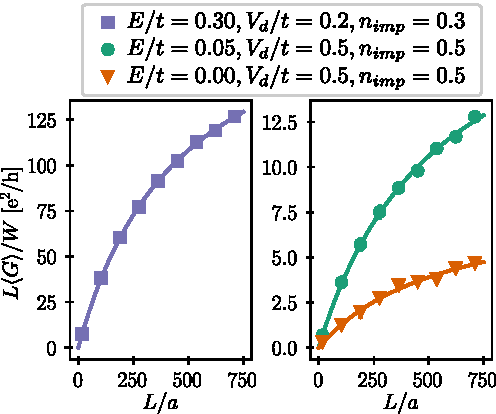
\includegraphics[width=0.95\columnwidth]{fig4}
%    \caption{Real-space visualization of the trajectory of $\bb{m}$ at different driving frequencies $\omega$, corresponding to the top panel in Fig.~\ref{fig:dynamics}}
%    \label{fig:sbloch}
%\end{figure}

In the regime of $\alpha_\textrm{G}\ll f_0 \ll \ll \omega_0$ we can find the asymptotic behavior of $m_\textrm{H}$ at sufficiently small times. In order to do that it is convenient to represnt $\bb{m}$ in spherical coordinates: $\bb{m}=(\sin\theta\cos\phi,\sin\theta\sin\phi,\cos\theta)^\top$, where $\theta$ is the polar angle between $\bb{m}$ and $\hat{\bb{z}}$ and $\phi$ is the azimuth. In the limit $\alpha_\textrm{G}\rightarrow 0$ we find the equations of motion on $\theta$ and $\phi$:
\begin{align}
\partial_t \theta &= \sin \chi  \sin \phi  f(\bb{r},t) \big(\sin \chi  \sin \theta \cos \phi -\cos \chi  \cos \theta \big)\\
\partial_t \phi &=\omega_0+f(r,t) 
  \cos\theta\big(\cos ^2\chi  \cos ^2\phi-\sin^2\phi -\frac{1}{2}\sin\chi(\cot\theta-\sin\theta) \big).
\end{align}
We take $f(\bb{r},t)=f_0\cos\omega t$ and assume that $f_0\ll\omega_0$, so that we find $\phi = \omega_0 t-\phi_0$. It is convenient to choose $\phi_0=\pi/2$ so that
\begin{align}
  \partial_t \theta = -f_0 \sin \chi  \cos ^2\omega_0t\,(\sin \theta  \sin \chi  \sin \omega_0t-\cos \theta  \cos \chi ).
  \label{chap1:eq:theta2}
\end{align}
Because we assumed that $f_0\ll\omega_0$, the dynamics of $\phi$ is much faster than the dynamics of $\theta$. Therefore we average Eq.~(\ref{chap1:eq:theta2}) over $\phi$ and obtain
\begin{equation}
  \partial_t\theta = \frac{f_0}{4} \cos \theta \sin2\chi.
\end{equation}
This equation is readily solved by means of the substitution $\cos\theta = 1/\cosh x$, $\sin\theta=-\tanh x$. Using the initial condition $\theta(0)=0$ one finds 
\begin{equation}
\cos\theta(t) = \frac{1}{\cosh\lt( \frac{1}{4}f_0 t \sin2\chi\rt)},
\end{equation}
which gives the result of Eq.~(\ref{asymptot}) of the main text.

%merlin.mbs apsrev4-1.bst 2010-07-25 4.21a (PWD, AO, DPC) hacked
%Control: key (0)
%Control: author (72) initials jnrlst
%Control: editor formatted (1) identically to author
%Control: production of article title (-1) disabled
%Control: page (0) single
%Control: year (1) truncated
%Control: production of eprint (0) enabled
% \begin{thebibliography}{69}%
% \makeatletter
% \providecommand \@ifxundefined [1]{%
%  \@ifx{#1\undefined}
% }%
% \providecommand \@ifnum [1]{%
%  \ifnum #1\expandafter \@firstoftwo
%  \else \expandafter \@secondoftwo
%  \fi
% }%
% \providecommand \@ifx [1]{%
%  \ifx #1\expandafter \@firstoftwo
%  \else \expandafter \@secondoftwo
%  \fi
% }%
% \providecommand \natexlab [1]{#1}%
% \providecommand \enquote  [1]{``#1''}%
% \providecommand \bibnamefont  [1]{#1}%
% \providecommand \bibfnamefont [1]{#1}%
% \providecommand \citenamefont [1]{#1}%
% \providecommand \href@noop [0]{\@secondoftwo}%
% \providecommand \href [0]{\begingroup \@sanitize@url \@href}%
% \providecommand \@href[1]{\@@startlink{#1}\@@href}%
% \providecommand \@@href[1]{\endgroup#1\@@endlink}%
% \providecommand \@sanitize@url [0]{\catcode `\\12\catcode `\$12\catcode
%   `\&12\catcode `\#12\catcode `\^12\catcode `\_12\catcode `\%12\relax}%
% \providecommand \@@startlink[1]{}%
% \providecommand \@@endlink[0]{}%
% \providecommand \url  [0]{\begingroup\@sanitize@url \@url }%
% \providecommand \@url [1]{\endgroup\@href {#1}{\urlprefix }}%
% \providecommand \urlprefix  [0]{URL }%
% \providecommand \Eprint [0]{\href }%
% \providecommand \doibase [0]{http://dx.doi.org/}%
% \providecommand \selectlanguage [0]{\@gobble}%
% \providecommand \bibinfo  [0]{\@secondoftwo}%
% \providecommand \bibfield  [0]{\@secondoftwo}%
% \providecommand \translation [1]{[#1]}%
% \providecommand \BibitemOpen [0]{}%
% \providecommand \bibitemStop [0]{}%
% \providecommand \bibitemNoStop [0]{.\EOS\space}%
% \providecommand \EOS [0]{\spacefactor3000\relax}%
% \providecommand \BibitemShut  [1]{\csname bibitem#1\endcsname}%
% \let\auto@bib@innerbib\@empty
% %</preamble>
% \bibitem [{\citenamefont {Miron}\ \emph {et~al.}(2010)\citenamefont {Miron},
%   \citenamefont {Gaudin}, \citenamefont {Auffret}, \citenamefont {Rodmacq},
%   \citenamefont {Schuhl}, \citenamefont {Pizzini}, \citenamefont {Vogel},\ and\
%   \citenamefont {Gambardella}}]{miron_current-driven_2010}%
%   \BibitemOpen
%   \bibfield  {author} {\bibinfo {author} {\bibfnamefont {I.~M.}\ \bibnamefont
%   {Miron}}, \bibinfo {author} {\bibfnamefont {G.}~\bibnamefont {Gaudin}},
%   \bibinfo {author} {\bibfnamefont {S.}~\bibnamefont {Auffret}}, \bibinfo
%   {author} {\bibfnamefont {B.}~\bibnamefont {Rodmacq}}, \bibinfo {author}
%   {\bibfnamefont {A.}~\bibnamefont {Schuhl}}, \bibinfo {author} {\bibfnamefont
%   {S.}~\bibnamefont {Pizzini}}, \bibinfo {author} {\bibfnamefont
%   {J.}~\bibnamefont {Vogel}}, \ and\ \bibinfo {author} {\bibfnamefont
%   {P.}~\bibnamefont {Gambardella}},\ }\href {\doibase 10.1038/nmat2613}
%   {\bibfield  {journal} {\bibinfo  {journal} {Nature Materials}\ }\textbf
%   {\bibinfo {volume} {9}},\ \bibinfo {pages} {230} (\bibinfo {year}
%   {2010})}\BibitemShut {NoStop}%
% \bibitem [{\citenamefont {Haney}\ \emph {et~al.}(2013)\citenamefont {Haney},
%   \citenamefont {Lee}, \citenamefont {Lee}, \citenamefont {Manchon},\ and\
%   \citenamefont {Stiles}}]{haney_current_2013}%
%   \BibitemOpen
%   \bibfield  {author} {\bibinfo {author} {\bibfnamefont {P.~M.}\ \bibnamefont
%   {Haney}}, \bibinfo {author} {\bibfnamefont {H.-W.}\ \bibnamefont {Lee}},
%   \bibinfo {author} {\bibfnamefont {K.-J.}\ \bibnamefont {Lee}}, \bibinfo
%   {author} {\bibfnamefont {A.}~\bibnamefont {Manchon}}, \ and\ \bibinfo
%   {author} {\bibfnamefont {M.~D.}\ \bibnamefont {Stiles}},\ }\href {\doibase
%   10.1103/PhysRevB.87.174411} {\bibfield  {journal} {\bibinfo  {journal} {Phys.
%   Rev. B}\ }\textbf {\bibinfo {volume} {87}} (\bibinfo {year} {2013}),\
%   10.1103/PhysRevB.87.174411}\BibitemShut {NoStop}%
% \bibitem [{\citenamefont {Dyakonov}\ and\ \citenamefont
%   {Perel}(1971)}]{dyakonov_current-induced_1971}%
%   \BibitemOpen
%   \bibfield  {author} {\bibinfo {author} {\bibfnamefont {M.~I.}\ \bibnamefont
%   {Dyakonov}}\ and\ \bibinfo {author} {\bibfnamefont {V.~I.}\ \bibnamefont
%   {Perel}},\ }\href {\doibase 10.1016/0375-9601(71)90196-4} {\bibfield
%   {journal} {\bibinfo  {journal} {Physics Letters A}\ }\textbf {\bibinfo
%   {volume} {35}},\ \bibinfo {pages} {459} (\bibinfo {year} {1971})}\BibitemShut
%   {NoStop}%
% \bibitem [{\citenamefont {Awschalom}\ and\ \citenamefont
%   {Samarth}(2009)}]{awschalom2009trend}%
%   \BibitemOpen
%   \bibfield  {author} {\bibinfo {author} {\bibfnamefont {D.}~\bibnamefont
%   {Awschalom}}\ and\ \bibinfo {author} {\bibfnamefont {N.}~\bibnamefont
%   {Samarth}},\ }\href@noop {} {\bibfield  {journal} {\bibinfo  {journal}
%   {Physics}\ }\textbf {\bibinfo {volume} {2}},\ \bibinfo {pages} {50} (\bibinfo
%   {year} {2009})}\BibitemShut {NoStop}%
% \bibitem [{\citenamefont {Manchon}\ and\ \citenamefont
%   {Zhang}(2008)}]{manchon_theory_2008}%
%   \BibitemOpen
%   \bibfield  {author} {\bibinfo {author} {\bibfnamefont {A.}~\bibnamefont
%   {Manchon}}\ and\ \bibinfo {author} {\bibfnamefont {S.}~\bibnamefont
%   {Zhang}},\ }\href {\doibase 10.1103/PhysRevB.78.212405} {\bibfield  {journal}
%   {\bibinfo  {journal} {Phys. Rev. B}\ }\textbf {\bibinfo {volume} {78}}
%   (\bibinfo {year} {2008}),\ 10.1103/PhysRevB.78.212405}\BibitemShut {NoStop}%
% \bibitem [{\citenamefont {Garate}\ and\ \citenamefont
%   {MacDonald}(2009)}]{garate_influence_2009}%
%   \BibitemOpen
%   \bibfield  {author} {\bibinfo {author} {\bibfnamefont {I.}~\bibnamefont
%   {Garate}}\ and\ \bibinfo {author} {\bibfnamefont {A.~H.}\ \bibnamefont
%   {MacDonald}},\ }\href {\doibase 10.1103/PhysRevB.80.134403} {\bibfield
%   {journal} {\bibinfo  {journal} {Phys. Rev. B}\ }\textbf {\bibinfo {volume}
%   {80}} (\bibinfo {year} {2009}),\ 10.1103/PhysRevB.80.134403}\BibitemShut
%   {NoStop}%
% \bibitem [{\citenamefont {Manchon}\ and\ \citenamefont
%   {Zhang}(2009)}]{manchon2009theory}%
%   \BibitemOpen
%   \bibfield  {author} {\bibinfo {author} {\bibfnamefont {A.}~\bibnamefont
%   {Manchon}}\ and\ \bibinfo {author} {\bibfnamefont {S.}~\bibnamefont
%   {Zhang}},\ }\href@noop {} {\bibfield  {journal} {\bibinfo  {journal}
%   {Physical Review B}\ }\textbf {\bibinfo {volume} {79}},\ \bibinfo {pages}
%   {094422} (\bibinfo {year} {2009})}\BibitemShut {NoStop}%
% \bibitem [{\citenamefont
%   {Slonczewski}(1996)}]{slonczewski_current-driven_1996}%
%   \BibitemOpen
%   \bibfield  {author} {\bibinfo {author} {\bibfnamefont {J.~C.}\ \bibnamefont
%   {Slonczewski}},\ }\href
%   {http://www.sciencedirect.com/science/article/pii/0304885396000625}
%   {\bibfield  {journal} {\bibinfo  {journal} {J. Magn. Magn. Mater.}\ }\textbf
%   {\bibinfo {volume} {159}},\ \bibinfo {pages} {L1} (\bibinfo {year}
%   {1996})}\BibitemShut {NoStop}%
% \bibitem [{\citenamefont {Berger}(1996)}]{berger_emission_1996}%
%   \BibitemOpen
%   \bibfield  {author} {\bibinfo {author} {\bibfnamefont {L.}~\bibnamefont
%   {Berger}},\ }\href
%   {https://journals.aps.org/prb/abstract/10.1103/PhysRevB.54.9353} {\bibfield
%   {journal} {\bibinfo  {journal} {Phys. Rev. B}\ }\textbf {\bibinfo {volume}
%   {54}},\ \bibinfo {pages} {9353} (\bibinfo {year} {1996})}\BibitemShut
%   {NoStop}%
% \bibitem [{\citenamefont {Ralph}\ and\ \citenamefont
%   {Stiles}(2008)}]{ralph_spin_2008}%
%   \BibitemOpen
%   \bibfield  {author} {\bibinfo {author} {\bibfnamefont {D.}~\bibnamefont
%   {Ralph}}\ and\ \bibinfo {author} {\bibfnamefont {M.}~\bibnamefont {Stiles}},\
%   }\href {\doibase 10.1016/j.jmmm.2007.12.019} {\bibfield  {journal} {\bibinfo
%   {journal} {Journal of Magnetism and Magnetic Materials}\ }\textbf {\bibinfo
%   {volume} {320}},\ \bibinfo {pages} {1190} (\bibinfo {year}
%   {2008})}\BibitemShut {NoStop}%
% \bibitem [{\citenamefont {Stiles}\ and\ \citenamefont
%   {Zangwill}(2002)}]{stiles_anatomy_2002}%
%   \BibitemOpen
%   \bibfield  {author} {\bibinfo {author} {\bibfnamefont {M.~D.}\ \bibnamefont
%   {Stiles}}\ and\ \bibinfo {author} {\bibfnamefont {A.}~\bibnamefont
%   {Zangwill}},\ }\href {\doibase 10.1103/PhysRevB.66.014407} {\bibfield
%   {journal} {\bibinfo  {journal} {Physical Review B}\ }\textbf {\bibinfo
%   {volume} {66}},\ \bibinfo {pages} {014407} (\bibinfo {year}
%   {2002})}\BibitemShut {NoStop}%
% \bibitem [{\citenamefont {Fu}\ \emph {et~al.}(2007)\citenamefont {Fu},
%   \citenamefont {Kane},\ and\ \citenamefont {Mele}}]{fu_topological_2007}%
%   \BibitemOpen
%   \bibfield  {author} {\bibinfo {author} {\bibfnamefont {L.}~\bibnamefont
%   {Fu}}, \bibinfo {author} {\bibfnamefont {C.~L.}\ \bibnamefont {Kane}}, \ and\
%   \bibinfo {author} {\bibfnamefont {E.~J.}\ \bibnamefont {Mele}},\ }\href
%   {\doibase 10.1103/PhysRevLett.98.106803} {\bibfield  {journal} {\bibinfo
%   {journal} {Physical Review Letters}\ }\textbf {\bibinfo {volume} {98}},\
%   \bibinfo {pages} {106803} (\bibinfo {year} {2007})}\BibitemShut {NoStop}%
% \bibitem [{\citenamefont {Moore}\ and\ \citenamefont
%   {Balents}(2007)}]{moore_topological_2007}%
%   \BibitemOpen
%   \bibfield  {author} {\bibinfo {author} {\bibfnamefont {J.~E.}\ \bibnamefont
%   {Moore}}\ and\ \bibinfo {author} {\bibfnamefont {L.}~\bibnamefont
%   {Balents}},\ }\href {\doibase 10.1103/PhysRevB.75.121306} {\bibfield
%   {journal} {\bibinfo  {journal} {Physical Review B}\ }\textbf {\bibinfo
%   {volume} {75}},\ \bibinfo {pages} {121306} (\bibinfo {year}
%   {2007})}\BibitemShut {NoStop}%
% \bibitem [{\citenamefont {Roy}(2009)}]{roy_topological_2009}%
%   \BibitemOpen
%   \bibfield  {author} {\bibinfo {author} {\bibfnamefont {R.}~\bibnamefont
%   {Roy}},\ }\href {\doibase 10.1103/PhysRevB.79.195322} {\bibfield  {journal}
%   {\bibinfo  {journal} {Physical Review B}\ }\textbf {\bibinfo {volume} {79}},\
%   \bibinfo {pages} {195322} (\bibinfo {year} {2009})}\BibitemShut {NoStop}%
% \bibitem [{\citenamefont {Hsieh}\ \emph {et~al.}(2008)\citenamefont {Hsieh},
%   \citenamefont {Qian}, \citenamefont {Wray}, \citenamefont {Xia},
%   \citenamefont {Hor}, \citenamefont {Cava},\ and\ \citenamefont
%   {Hasan}}]{hsieh_topological_2008}%
%   \BibitemOpen
%   \bibfield  {author} {\bibinfo {author} {\bibfnamefont {D.}~\bibnamefont
%   {Hsieh}}, \bibinfo {author} {\bibfnamefont {D.}~\bibnamefont {Qian}},
%   \bibinfo {author} {\bibfnamefont {L.}~\bibnamefont {Wray}}, \bibinfo {author}
%   {\bibfnamefont {Y.}~\bibnamefont {Xia}}, \bibinfo {author} {\bibfnamefont
%   {Y.~S.}\ \bibnamefont {Hor}}, \bibinfo {author} {\bibfnamefont {R.~J.}\
%   \bibnamefont {Cava}}, \ and\ \bibinfo {author} {\bibfnamefont {M.~Z.}\
%   \bibnamefont {Hasan}},\ }\href {\doibase 10.1038/nature06843} {\bibfield
%   {journal} {\bibinfo  {journal} {Nature}\ }\textbf {\bibinfo {volume} {452}},\
%   \bibinfo {pages} {970} (\bibinfo {year} {2008})}\BibitemShut {NoStop}%
% \bibitem [{\citenamefont {Qi}\ \emph {et~al.}(2008{\natexlab{a}})\citenamefont
%   {Qi}, \citenamefont {Hughes},\ and\ \citenamefont
%   {Zhang}}]{qi_fractional_2008}%
%   \BibitemOpen
%   \bibfield  {author} {\bibinfo {author} {\bibfnamefont {X.-L.}\ \bibnamefont
%   {Qi}}, \bibinfo {author} {\bibfnamefont {T.~L.}\ \bibnamefont {Hughes}}, \
%   and\ \bibinfo {author} {\bibfnamefont {S.-C.}\ \bibnamefont {Zhang}},\ }\href
%   {\doibase 10.1038/nphys913} {\bibfield  {journal} {\bibinfo  {journal}
%   {Nature Physics}\ }\textbf {\bibinfo {volume} {4}},\ \bibinfo {pages} {273}
%   (\bibinfo {year} {2008}{\natexlab{a}})}\BibitemShut {NoStop}%
% \bibitem [{\citenamefont {Mellnik}\ \emph {et~al.}(2014)\citenamefont
%   {Mellnik}, \citenamefont {Lee}, \citenamefont {Richardella}, \citenamefont
%   {Grab}, \citenamefont {Mintun}, \citenamefont {Fischer}, \citenamefont
%   {Vaezi}, \citenamefont {Manchon}, \citenamefont {Kim}, \citenamefont
%   {Samarth},\ and\ \citenamefont {Ralph}}]{mellnik_spin-transfer_2014}%
%   \BibitemOpen
%   \bibfield  {author} {\bibinfo {author} {\bibfnamefont {A.~R.}\ \bibnamefont
%   {Mellnik}}, \bibinfo {author} {\bibfnamefont {J.~S.}\ \bibnamefont {Lee}},
%   \bibinfo {author} {\bibfnamefont {A.}~\bibnamefont {Richardella}}, \bibinfo
%   {author} {\bibfnamefont {J.~L.}\ \bibnamefont {Grab}}, \bibinfo {author}
%   {\bibfnamefont {P.~J.}\ \bibnamefont {Mintun}}, \bibinfo {author}
%   {\bibfnamefont {M.~H.}\ \bibnamefont {Fischer}}, \bibinfo {author}
%   {\bibfnamefont {A.}~\bibnamefont {Vaezi}}, \bibinfo {author} {\bibfnamefont
%   {A.}~\bibnamefont {Manchon}}, \bibinfo {author} {\bibfnamefont {E.-A.}\
%   \bibnamefont {Kim}}, \bibinfo {author} {\bibfnamefont {N.}~\bibnamefont
%   {Samarth}}, \ and\ \bibinfo {author} {\bibfnamefont {D.~C.}\ \bibnamefont
%   {Ralph}},\ }\href {\doibase 10.1038/nature13534} {\bibfield  {journal}
%   {\bibinfo  {journal} {Nature}\ }\textbf {\bibinfo {volume} {511}},\ \bibinfo
%   {pages} {449} (\bibinfo {year} {2014})}\BibitemShut {NoStop}%
% \bibitem [{\citenamefont {Wang}\ \emph {et~al.}(2015)\citenamefont {Wang},
%   \citenamefont {Deorani}, \citenamefont {Banerjee}, \citenamefont {Koirala},
%   \citenamefont {Brahlek}, \citenamefont {Oh},\ and\ \citenamefont
%   {Yang}}]{wang_SOT_BiSe_2014}%
%   \BibitemOpen
%   \bibfield  {author} {\bibinfo {author} {\bibfnamefont {Y.}~\bibnamefont
%   {Wang}}, \bibinfo {author} {\bibfnamefont {P.}~\bibnamefont {Deorani}},
%   \bibinfo {author} {\bibfnamefont {K.}~\bibnamefont {Banerjee}}, \bibinfo
%   {author} {\bibfnamefont {N.}~\bibnamefont {Koirala}}, \bibinfo {author}
%   {\bibfnamefont {M.}~\bibnamefont {Brahlek}}, \bibinfo {author} {\bibfnamefont
%   {S.}~\bibnamefont {Oh}}, \ and\ \bibinfo {author} {\bibfnamefont
%   {H.}~\bibnamefont {Yang}},\ }\href {\doibase 10.1103/PhysRevLett.114.257202}
%   {\bibfield  {journal} {\bibinfo  {journal} {Phys. Rev. Lett.}\ }\textbf
%   {\bibinfo {volume} {114}},\ \bibinfo {pages} {257202} (\bibinfo {year}
%   {2015})}\BibitemShut {NoStop}%
% \bibitem [{\citenamefont {Fan}\ \emph {et~al.}(2014)\citenamefont {Fan},
%   \citenamefont {Upadhyaya}, \citenamefont {Kou}, \citenamefont {Lang},
%   \citenamefont {Takei}, \citenamefont {Wang}, \citenamefont {Tang},
%   \citenamefont {He}, \citenamefont {Chang}, \citenamefont {Montazeri},
%   \citenamefont {Yu}, \citenamefont {Jiang}, \citenamefont {Nie}, \citenamefont
%   {Schwartz}, \citenamefont {Tserkovnyak},\ and\ \citenamefont
%   {Wang}}]{fan_magnetization_2014}%
%   \BibitemOpen
%   \bibfield  {author} {\bibinfo {author} {\bibfnamefont {Y.}~\bibnamefont
%   {Fan}}, \bibinfo {author} {\bibfnamefont {P.}~\bibnamefont {Upadhyaya}},
%   \bibinfo {author} {\bibfnamefont {X.}~\bibnamefont {Kou}}, \bibinfo {author}
%   {\bibfnamefont {M.}~\bibnamefont {Lang}}, \bibinfo {author} {\bibfnamefont
%   {S.}~\bibnamefont {Takei}}, \bibinfo {author} {\bibfnamefont
%   {Z.}~\bibnamefont {Wang}}, \bibinfo {author} {\bibfnamefont {J.}~\bibnamefont
%   {Tang}}, \bibinfo {author} {\bibfnamefont {L.}~\bibnamefont {He}}, \bibinfo
%   {author} {\bibfnamefont {L.-T.}\ \bibnamefont {Chang}}, \bibinfo {author}
%   {\bibfnamefont {M.}~\bibnamefont {Montazeri}}, \bibinfo {author}
%   {\bibfnamefont {G.}~\bibnamefont {Yu}}, \bibinfo {author} {\bibfnamefont
%   {W.}~\bibnamefont {Jiang}}, \bibinfo {author} {\bibfnamefont
%   {T.}~\bibnamefont {Nie}}, \bibinfo {author} {\bibfnamefont {R.~N.}\
%   \bibnamefont {Schwartz}}, \bibinfo {author} {\bibfnamefont {Y.}~\bibnamefont
%   {Tserkovnyak}}, \ and\ \bibinfo {author} {\bibfnamefont {K.~L.}\ \bibnamefont
%   {Wang}},\ }\href {\doibase 10.1038/nmat3973} {\bibfield  {journal} {\bibinfo
%   {journal} {Nature Materials}\ }\textbf {\bibinfo {volume} {13}},\ \bibinfo
%   {pages} {699} (\bibinfo {year} {2014})}\BibitemShut {NoStop}%
% \bibitem [{\citenamefont {Fan}\ \emph {et~al.}(2016)\citenamefont {Fan},
%   \citenamefont {Kou}, \citenamefont {Upadhyaya}, \citenamefont {Shao},
%   \citenamefont {Pan}, \citenamefont {Lang}, \citenamefont {Che}, \citenamefont
%   {Tang}, \citenamefont {Montazeri}, \citenamefont {Murata}, \citenamefont
%   {Chang}, \citenamefont {Akyol}, \citenamefont {Yu}, \citenamefont {Nie},
%   \citenamefont {Wong}, \citenamefont {Liu}, \citenamefont {Wang},
%   \citenamefont {Tserkovnyak},\ and\ \citenamefont {Wang}}]{Fan_SOT_TI_2016}%
%   \BibitemOpen
%   \bibfield  {author} {\bibinfo {author} {\bibfnamefont {Y.}~\bibnamefont
%   {Fan}}, \bibinfo {author} {\bibfnamefont {X.}~\bibnamefont {Kou}}, \bibinfo
%   {author} {\bibfnamefont {P.}~\bibnamefont {Upadhyaya}}, \bibinfo {author}
%   {\bibfnamefont {Q.}~\bibnamefont {Shao}}, \bibinfo {author} {\bibfnamefont
%   {L.}~\bibnamefont {Pan}}, \bibinfo {author} {\bibfnamefont {M.}~\bibnamefont
%   {Lang}}, \bibinfo {author} {\bibfnamefont {X.}~\bibnamefont {Che}}, \bibinfo
%   {author} {\bibfnamefont {J.}~\bibnamefont {Tang}}, \bibinfo {author}
%   {\bibfnamefont {M.}~\bibnamefont {Montazeri}}, \bibinfo {author}
%   {\bibfnamefont {K.}~\bibnamefont {Murata}}, \bibinfo {author} {\bibfnamefont
%   {L.-T.}\ \bibnamefont {Chang}}, \bibinfo {author} {\bibfnamefont
%   {M.}~\bibnamefont {Akyol}}, \bibinfo {author} {\bibfnamefont
%   {G.}~\bibnamefont {Yu}}, \bibinfo {author} {\bibfnamefont {T.}~\bibnamefont
%   {Nie}}, \bibinfo {author} {\bibfnamefont {K.~L.}\ \bibnamefont {Wong}},
%   \bibinfo {author} {\bibfnamefont {J.}~\bibnamefont {Liu}}, \bibinfo {author}
%   {\bibfnamefont {Y.}~\bibnamefont {Wang}}, \bibinfo {author} {\bibfnamefont
%   {Y.}~\bibnamefont {Tserkovnyak}}, \ and\ \bibinfo {author} {\bibfnamefont
%   {K.~L.}\ \bibnamefont {Wang}},\ }\href
%   {http://dx.doi.org/10.1038/nnano.2015.294} {\bibfield  {journal} {\bibinfo
%   {journal} {Nature Nanotechnology}\ }\textbf {\bibinfo {volume} {11}},\
%   \bibinfo {pages} {352 EP } (\bibinfo {year} {2016})}\BibitemShut {NoStop}%
% \bibitem [{\citenamefont {Yasuda}\ \emph {et~al.}(2017)\citenamefont {Yasuda},
%   \citenamefont {Tsukazaki}, \citenamefont {Yoshimi}, \citenamefont {Kondou},
%   \citenamefont {Takahashi}, \citenamefont {Otani}, \citenamefont {Kawasaki},\
%   and\ \citenamefont {Tokura}}]{Yasuda_SOT_BiSbTe_2017}%
%   \BibitemOpen
%   \bibfield  {author} {\bibinfo {author} {\bibfnamefont {K.}~\bibnamefont
%   {Yasuda}}, \bibinfo {author} {\bibfnamefont {A.}~\bibnamefont {Tsukazaki}},
%   \bibinfo {author} {\bibfnamefont {R.}~\bibnamefont {Yoshimi}}, \bibinfo
%   {author} {\bibfnamefont {K.}~\bibnamefont {Kondou}}, \bibinfo {author}
%   {\bibfnamefont {K.~S.}\ \bibnamefont {Takahashi}}, \bibinfo {author}
%   {\bibfnamefont {Y.}~\bibnamefont {Otani}}, \bibinfo {author} {\bibfnamefont
%   {M.}~\bibnamefont {Kawasaki}}, \ and\ \bibinfo {author} {\bibfnamefont
%   {Y.}~\bibnamefont {Tokura}},\ }\href {\doibase
%   10.1103/PhysRevLett.119.137204} {\bibfield  {journal} {\bibinfo  {journal}
%   {Phys. Rev. Lett.}\ }\textbf {\bibinfo {volume} {119}},\ \bibinfo {pages}
%   {137204} (\bibinfo {year} {2017})}\BibitemShut {NoStop}%
% \bibitem [{\citenamefont {Cha}\ \emph {et~al.}(2018)\citenamefont {Cha},
%   \citenamefont {Noh}, \citenamefont {Kim}, \citenamefont {Son}, \citenamefont
%   {Bae}, \citenamefont {Lee}, \citenamefont {Kim}, \citenamefont {Lee},
%   \citenamefont {Shin}, \citenamefont {Sim}, \citenamefont {Yang},
%   \citenamefont {Lee}, \citenamefont {Shim}, \citenamefont {Lee}, \citenamefont
%   {Jo}, \citenamefont {Kim}, \citenamefont {Kim},\ and\ \citenamefont
%   {Choi}}]{Cha2018}%
%   \BibitemOpen
%   \bibfield  {author} {\bibinfo {author} {\bibfnamefont {S.}~\bibnamefont
%   {Cha}}, \bibinfo {author} {\bibfnamefont {M.}~\bibnamefont {Noh}}, \bibinfo
%   {author} {\bibfnamefont {J.}~\bibnamefont {Kim}}, \bibinfo {author}
%   {\bibfnamefont {J.}~\bibnamefont {Son}}, \bibinfo {author} {\bibfnamefont
%   {H.}~\bibnamefont {Bae}}, \bibinfo {author} {\bibfnamefont {D.}~\bibnamefont
%   {Lee}}, \bibinfo {author} {\bibfnamefont {H.}~\bibnamefont {Kim}}, \bibinfo
%   {author} {\bibfnamefont {J.}~\bibnamefont {Lee}}, \bibinfo {author}
%   {\bibfnamefont {H.-S.}\ \bibnamefont {Shin}}, \bibinfo {author}
%   {\bibfnamefont {S.}~\bibnamefont {Sim}}, \bibinfo {author} {\bibfnamefont
%   {S.}~\bibnamefont {Yang}}, \bibinfo {author} {\bibfnamefont {S.}~\bibnamefont
%   {Lee}}, \bibinfo {author} {\bibfnamefont {W.}~\bibnamefont {Shim}}, \bibinfo
%   {author} {\bibfnamefont {C.-H.}\ \bibnamefont {Lee}}, \bibinfo {author}
%   {\bibfnamefont {M.-H.}\ \bibnamefont {Jo}}, \bibinfo {author} {\bibfnamefont
%   {J.~S.}\ \bibnamefont {Kim}}, \bibinfo {author} {\bibfnamefont
%   {D.}~\bibnamefont {Kim}}, \ and\ \bibinfo {author} {\bibfnamefont
%   {H.}~\bibnamefont {Choi}},\ }\href {\doibase 10.1038/s41565-018-0195-y}
%   {\bibfield  {journal} {\bibinfo  {journal} {Nature Nanotechnology}\ }
%   (\bibinfo {year} {2018}),\ 10.1038/s41565-018-0195-y}\BibitemShut {NoStop}%
% \bibitem [{\citenamefont {Liu}\ \emph {et~al.}(2011)\citenamefont {Liu},
%   \citenamefont {Moriyama}, \citenamefont {Ralph},\ and\ \citenamefont
%   {Buhrman}}]{Ralph2011SOTFMresonance}%
%   \BibitemOpen
%   \bibfield  {author} {\bibinfo {author} {\bibfnamefont {L.}~\bibnamefont
%   {Liu}}, \bibinfo {author} {\bibfnamefont {T.}~\bibnamefont {Moriyama}},
%   \bibinfo {author} {\bibfnamefont {D.~C.}\ \bibnamefont {Ralph}}, \ and\
%   \bibinfo {author} {\bibfnamefont {R.~A.}\ \bibnamefont {Buhrman}},\ }\href
%   {\doibase 10.1103/PhysRevLett.106.036601} {\bibfield  {journal} {\bibinfo
%   {journal} {Phys. Rev. Lett.}\ }\textbf {\bibinfo {volume} {106}},\ \bibinfo
%   {pages} {036601} (\bibinfo {year} {2011})}\BibitemShut {NoStop}%
% \bibitem [{\citenamefont {Akyol}\ \emph {et~al.}(2015)\citenamefont {Akyol},
%   \citenamefont {Yu}, \citenamefont {Alzate}, \citenamefont {Upadhyaya},
%   \citenamefont {Li}, \citenamefont {Wong}, \citenamefont {Ekicibil},
%   \citenamefont {Khalili~Amiri},\ and\ \citenamefont
%   {Wang}}]{Wang2015_SOTHflCoFEBIMgO}%
%   \BibitemOpen
%   \bibfield  {author} {\bibinfo {author} {\bibfnamefont {M.}~\bibnamefont
%   {Akyol}}, \bibinfo {author} {\bibfnamefont {G.}~\bibnamefont {Yu}}, \bibinfo
%   {author} {\bibfnamefont {J.~G.}\ \bibnamefont {Alzate}}, \bibinfo {author}
%   {\bibfnamefont {P.}~\bibnamefont {Upadhyaya}}, \bibinfo {author}
%   {\bibfnamefont {X.}~\bibnamefont {Li}}, \bibinfo {author} {\bibfnamefont
%   {K.~L.}\ \bibnamefont {Wong}}, \bibinfo {author} {\bibfnamefont
%   {A.}~\bibnamefont {Ekicibil}}, \bibinfo {author} {\bibfnamefont
%   {P.}~\bibnamefont {Khalili~Amiri}}, \ and\ \bibinfo {author} {\bibfnamefont
%   {K.~L.}\ \bibnamefont {Wang}},\ }\href {\doibase 10.1063/1.4919108}
%   {\bibfield  {journal} {\bibinfo  {journal} {Applied Physics Letters}\
%   }\textbf {\bibinfo {volume} {106}},\ \bibinfo {pages} {162409} (\bibinfo
%   {year} {2015})},\ \Eprint
%   {http://arxiv.org/abs/https://doi.org/10.1063/1.4919108}
%   {https://doi.org/10.1063/1.4919108} \BibitemShut {NoStop}%
% \bibitem [{\citenamefont {MacNeill}\ \emph {et~al.}(2016)\citenamefont
%   {MacNeill}, \citenamefont {Stiehl}, \citenamefont {Guimaraes}, \citenamefont
%   {Buhrman}, \citenamefont {Park},\ and\ \citenamefont
%   {Ralph}}]{Ralph2016SOTWTE2}%
%   \BibitemOpen
%   \bibfield  {author} {\bibinfo {author} {\bibfnamefont {D.}~\bibnamefont
%   {MacNeill}}, \bibinfo {author} {\bibfnamefont {G.~M.}\ \bibnamefont
%   {Stiehl}}, \bibinfo {author} {\bibfnamefont {M.~H.~D.}\ \bibnamefont
%   {Guimaraes}}, \bibinfo {author} {\bibfnamefont {R.~A.}\ \bibnamefont
%   {Buhrman}}, \bibinfo {author} {\bibfnamefont {J.}~\bibnamefont {Park}}, \
%   and\ \bibinfo {author} {\bibfnamefont {D.~C.}\ \bibnamefont {Ralph}},\ }\href
%   {https://doi.org/10.1038/nphys3933} {\bibfield  {journal} {\bibinfo
%   {journal} {Nature Physics}\ }\textbf {\bibinfo {volume} {13}},\ \bibinfo
%   {pages} {300 EP } (\bibinfo {year} {2016})}\BibitemShut {NoStop}%
% \bibitem [{\citenamefont {Guimaraes}\ \emph {et~al.}(2018)\citenamefont
%   {Guimaraes}, \citenamefont {Stiehl}, \citenamefont {MacNeill}, \citenamefont
%   {Reynolds},\ and\ \citenamefont {Ralph}}]{Ralph2018SOT}%
%   \BibitemOpen
%   \bibfield  {author} {\bibinfo {author} {\bibfnamefont {M.~H.~D.}\
%   \bibnamefont {Guimaraes}}, \bibinfo {author} {\bibfnamefont {G.~M.}\
%   \bibnamefont {Stiehl}}, \bibinfo {author} {\bibfnamefont {D.}~\bibnamefont
%   {MacNeill}}, \bibinfo {author} {\bibfnamefont {N.~D.}\ \bibnamefont
%   {Reynolds}}, \ and\ \bibinfo {author} {\bibfnamefont {D.~C.}\ \bibnamefont
%   {Ralph}},\ }\href {\doibase 10.1021/acs.nanolett.7b04993} {\bibfield
%   {journal} {\bibinfo  {journal} {Nano Letters}\ }\textbf {\bibinfo {volume}
%   {18}},\ \bibinfo {pages} {1311} (\bibinfo {year} {2018})},\ \bibinfo {note}
%   {pMID: 29328662},\ \Eprint
%   {http://arxiv.org/abs/https://doi.org/10.1021/acs.nanolett.7b04993}
%   {https://doi.org/10.1021/acs.nanolett.7b04993} \BibitemShut {NoStop}%
% \bibitem [{\citenamefont {Sakai}\ and\ \citenamefont
%   {Kohno}(2014)}]{sakai_spin_2014}%
%   \BibitemOpen
%   \bibfield  {author} {\bibinfo {author} {\bibfnamefont {A.}~\bibnamefont
%   {Sakai}}\ and\ \bibinfo {author} {\bibfnamefont {H.}~\bibnamefont {Kohno}},\
%   }\href {\doibase 10.1103/PhysRevB.89.165307} {\bibfield  {journal} {\bibinfo
%   {journal} {Physical Review B}\ }\textbf {\bibinfo {volume} {89}} (\bibinfo
%   {year} {2014}),\ 10.1103/PhysRevB.89.165307}\BibitemShut {NoStop}%
% \bibitem [{\citenamefont {Ndiaye}\ \emph {et~al.}(2017)\citenamefont {Ndiaye},
%   \citenamefont {Akosa}, \citenamefont {Fischer}, \citenamefont {Vaezi},
%   \citenamefont {Kim},\ and\ \citenamefont {Manchon}}]{ndiaye_dirac_2017}%
%   \BibitemOpen
%   \bibfield  {author} {\bibinfo {author} {\bibfnamefont {P.~B.}\ \bibnamefont
%   {Ndiaye}}, \bibinfo {author} {\bibfnamefont {C.~A.}\ \bibnamefont {Akosa}},
%   \bibinfo {author} {\bibfnamefont {M.~H.}\ \bibnamefont {Fischer}}, \bibinfo
%   {author} {\bibfnamefont {A.}~\bibnamefont {Vaezi}}, \bibinfo {author}
%   {\bibfnamefont {E.-A.}\ \bibnamefont {Kim}}, \ and\ \bibinfo {author}
%   {\bibfnamefont {A.}~\bibnamefont {Manchon}},\ }\href {\doibase
%   10.1103/ndiaye_dirac_2017} {\bibfield  {journal} {\bibinfo  {journal}
%   {Physical Review B}\ }\textbf {\bibinfo {volume} {96}} (\bibinfo {year}
%   {2017}),\ 10.1103/PhysRevB.96.014408}\BibitemShut {NoStop}%
% \bibitem [{\citenamefont {Burkov}\ and\ \citenamefont
%   {Hawthorn}(2010)}]{burkov_spin_2010-1}%
%   \BibitemOpen
%   \bibfield  {author} {\bibinfo {author} {\bibfnamefont {A.~A.}\ \bibnamefont
%   {Burkov}}\ and\ \bibinfo {author} {\bibfnamefont {D.~G.}\ \bibnamefont
%   {Hawthorn}},\ }\href {\doibase 10.1103/PhysRevLett.105.066802} {\bibfield
%   {journal} {\bibinfo  {journal} {Physical Review Letters}\ }\textbf {\bibinfo
%   {volume} {105}},\ \bibinfo {pages} {066802} (\bibinfo {year}
%   {2010})}\BibitemShut {NoStop}%
% \bibitem [{\citenamefont {Taguchi}\ \emph {et~al.}(2015)\citenamefont
%   {Taguchi}, \citenamefont {Shintani},\ and\ \citenamefont
%   {Tanaka}}]{taguchi_spin-charge_2015}%
%   \BibitemOpen
%   \bibfield  {author} {\bibinfo {author} {\bibfnamefont {K.}~\bibnamefont
%   {Taguchi}}, \bibinfo {author} {\bibfnamefont {K.}~\bibnamefont {Shintani}}, \
%   and\ \bibinfo {author} {\bibfnamefont {Y.}~\bibnamefont {Tanaka}},\ }\href
%   {\doibase 10.1103/PhysRevB.92.035425} {\bibfield  {journal} {\bibinfo
%   {journal} {Physical Review B}\ }\textbf {\bibinfo {volume} {92}} (\bibinfo
%   {year} {2015}),\ 10.1103/PhysRevB.92.035425}\BibitemShut {NoStop}%
% \bibitem [{\citenamefont {Shintani}\ \emph {et~al.}(2016)\citenamefont
%   {Shintani}, \citenamefont {Taguchi}, \citenamefont {Tanaka},\ and\
%   \citenamefont {Kawaguchi}}]{shintani_spin_2016}%
%   \BibitemOpen
%   \bibfield  {author} {\bibinfo {author} {\bibfnamefont {K.}~\bibnamefont
%   {Shintani}}, \bibinfo {author} {\bibfnamefont {K.}~\bibnamefont {Taguchi}},
%   \bibinfo {author} {\bibfnamefont {Y.}~\bibnamefont {Tanaka}}, \ and\ \bibinfo
%   {author} {\bibfnamefont {Y.}~\bibnamefont {Kawaguchi}},\ }\href {\doibase
%   10.1103/PhysRevB.93.195415} {\bibfield  {journal} {\bibinfo  {journal}
%   {Physical Review B}\ }\textbf {\bibinfo {volume} {93}},\ \bibinfo {pages}
%   {195415} (\bibinfo {year} {2016})}\BibitemShut {NoStop}%
% \bibitem [{\citenamefont {Vonsovsky}(1974)}]{sdmodel}%
%   \BibitemOpen
%   \bibfield  {author} {\bibinfo {author} {\bibfnamefont {S.~V.}\ \bibnamefont
%   {Vonsovsky}},\ }\href@noop {} {\emph {\bibinfo {title} {Magnetism}}}\
%   (\bibinfo  {publisher} {Wiley, New York},\ \bibinfo {year}
%   {1974})\BibitemShut {NoStop}%
% \bibitem [{\citenamefont {Ghosh}\ and\ \citenamefont
%   {Manchon}(2018)}]{Ghosh18}%
%   \BibitemOpen
%   \bibfield  {author} {\bibinfo {author} {\bibfnamefont {S.}~\bibnamefont
%   {Ghosh}}\ and\ \bibinfo {author} {\bibfnamefont {A.}~\bibnamefont
%   {Manchon}},\ }\href {\doibase 10.1103/PhysRevB.97.134402} {\bibfield
%   {journal} {\bibinfo  {journal} {Phys. Rev. B}\ }\textbf {\bibinfo {volume}
%   {97}},\ \bibinfo {pages} {134402} (\bibinfo {year} {2018})}\BibitemShut
%   {NoStop}%
% \bibitem [{\citenamefont {Maleev}\ and\ \citenamefont
%   {Toperverg}(1975)}]{maleev1975corrections}%
%   \BibitemOpen
%   \bibfield  {author} {\bibinfo {author} {\bibfnamefont {S.}~\bibnamefont
%   {Maleev}}\ and\ \bibinfo {author} {\bibfnamefont {B.}~\bibnamefont
%   {Toperverg}},\ }\href@noop {} {\bibfield  {journal} {\bibinfo  {journal} {Zh.
%   Eksp. Teor. Fiz}\ }\textbf {\bibinfo {volume} {69}},\ \bibinfo {pages} {1440}
%   (\bibinfo {year} {1975})}\BibitemShut {NoStop}%
% \bibitem [{\citenamefont {Maleev}\ and\ \citenamefont
%   {Toperverg}(1976)}]{maleev1976corrections}%
%   \BibitemOpen
%   \bibfield  {author} {\bibinfo {author} {\bibfnamefont {S.}~\bibnamefont
%   {Maleev}}\ and\ \bibinfo {author} {\bibfnamefont {B.}~\bibnamefont
%   {Toperverg}},\ }\href@noop {} {\bibfield  {journal} {\bibinfo  {journal}
%   {Soviet Journal of Experimental and Theoretical Physics}\ }\textbf {\bibinfo
%   {volume} {42}},\ \bibinfo {pages} {734} (\bibinfo {year} {1976})}\BibitemShut
%   {NoStop}%
% \bibitem [{\citenamefont {Altshuler}\ and\ \citenamefont
%   {Aronov}(1985)}]{altshuler1985electron}%
%   \BibitemOpen
%   \bibfield  {author} {\bibinfo {author} {\bibfnamefont {B.}~\bibnamefont
%   {Altshuler}}\ and\ \bibinfo {author} {\bibfnamefont {A.~G.}\ \bibnamefont
%   {Aronov}},\ }\href@noop {} {\bibfield  {journal} {\bibinfo  {journal}
%   {Amsterdam: North-Holland) p}\ }\textbf {\bibinfo {volume} {1}},\ \bibinfo
%   {pages} {155} (\bibinfo {year} {1985})}\BibitemShut {NoStop}%
% \bibitem [{\citenamefont {Ado}\ \emph {et~al.}(2015)\citenamefont {Ado},
%   \citenamefont {Dmitriev}, \citenamefont {Ostrovsky},\ and\ \citenamefont
%   {Titov}}]{ivanEPL}%
%   \BibitemOpen
%   \bibfield  {author} {\bibinfo {author} {\bibfnamefont {I.~A.}\ \bibnamefont
%   {Ado}}, \bibinfo {author} {\bibfnamefont {I.~A.}\ \bibnamefont {Dmitriev}},
%   \bibinfo {author} {\bibfnamefont {P.~M.}\ \bibnamefont {Ostrovsky}}, \ and\
%   \bibinfo {author} {\bibfnamefont {M.}~\bibnamefont {Titov}},\ }\href
%   {\doibase 10.1209/0295-5075/111/37004} {\bibfield  {journal} {\bibinfo
%   {journal} {EPL (Europhysics Letters)}\ }\textbf {\bibinfo {volume} {111}},\
%   \bibinfo {pages} {37004} (\bibinfo {year} {2015})}\BibitemShut {NoStop}%
% \bibitem [{\citenamefont {Ado}\ \emph {et~al.}(2016)\citenamefont {Ado},
%   \citenamefont {Dmitriev}, \citenamefont {Ostrovsky},\ and\ \citenamefont
%   {Titov}}]{ivanPRL}%
%   \BibitemOpen
%   \bibfield  {author} {\bibinfo {author} {\bibfnamefont {I.~A.}\ \bibnamefont
%   {Ado}}, \bibinfo {author} {\bibfnamefont {I.~A.}\ \bibnamefont {Dmitriev}},
%   \bibinfo {author} {\bibfnamefont {P.~M.}\ \bibnamefont {Ostrovsky}}, \ and\
%   \bibinfo {author} {\bibfnamefont {M.}~\bibnamefont {Titov}},\ }\href
%   {\doibase 10.1103/PhysRevLett.117.046601} {\bibfield  {journal} {\bibinfo
%   {journal} {Phys. Rev. Lett.}\ }\textbf {\bibinfo {volume} {117}},\ \bibinfo
%   {pages} {046601} (\bibinfo {year} {2016})}\BibitemShut {NoStop}%
% \bibitem [{\citenamefont {Ado}\ \emph {et~al.}(2017)\citenamefont {Ado},
%   \citenamefont {Dmitriev}, \citenamefont {Ostrovsky},\ and\ \citenamefont
%   {Titov}}]{ivanPRB}%
%   \BibitemOpen
%   \bibfield  {author} {\bibinfo {author} {\bibfnamefont {I.~A.}\ \bibnamefont
%   {Ado}}, \bibinfo {author} {\bibfnamefont {I.~A.}\ \bibnamefont {Dmitriev}},
%   \bibinfo {author} {\bibfnamefont {P.~M.}\ \bibnamefont {Ostrovsky}}, \ and\
%   \bibinfo {author} {\bibfnamefont {M.}~\bibnamefont {Titov}},\ }\href
%   {\doibase 10.1103/PhysRevB.96.235148} {\bibfield  {journal} {\bibinfo
%   {journal} {Phys. Rev. B}\ }\textbf {\bibinfo {volume} {96}},\ \bibinfo
%   {pages} {235148} (\bibinfo {year} {2017})}\BibitemShut {NoStop}%
% \bibitem [{\citenamefont {Kong}\ \emph {et~al.}(2011)\citenamefont {Kong},
%   \citenamefont {Cha}, \citenamefont {Lai}, \citenamefont {Peng}, \citenamefont
%   {Analytis}, \citenamefont {Meister}, \citenamefont {Chen}, \citenamefont
%   {Zhang}, \citenamefont {Fisher}, \citenamefont {Shen},\ and\ \citenamefont
%   {Cui}}]{kong_rapid_2011}%
%   \BibitemOpen
%   \bibfield  {author} {\bibinfo {author} {\bibfnamefont {D.}~\bibnamefont
%   {Kong}}, \bibinfo {author} {\bibfnamefont {J.~J.}\ \bibnamefont {Cha}},
%   \bibinfo {author} {\bibfnamefont {K.}~\bibnamefont {Lai}}, \bibinfo {author}
%   {\bibfnamefont {H.}~\bibnamefont {Peng}}, \bibinfo {author} {\bibfnamefont
%   {J.~G.}\ \bibnamefont {Analytis}}, \bibinfo {author} {\bibfnamefont
%   {S.}~\bibnamefont {Meister}}, \bibinfo {author} {\bibfnamefont
%   {Y.}~\bibnamefont {Chen}}, \bibinfo {author} {\bibfnamefont {H.-J.}\
%   \bibnamefont {Zhang}}, \bibinfo {author} {\bibfnamefont {I.~R.}\ \bibnamefont
%   {Fisher}}, \bibinfo {author} {\bibfnamefont {Z.-X.}\ \bibnamefont {Shen}}, \
%   and\ \bibinfo {author} {\bibfnamefont {Y.}~\bibnamefont {Cui}},\ }\href
%   {\doibase 10.1021/nn200556h} {\bibfield  {journal} {\bibinfo  {journal} {ACS
%   Nano}\ }\textbf {\bibinfo {volume} {5}},\ \bibinfo {pages} {4698} (\bibinfo
%   {year} {2011})}\BibitemShut {NoStop}%
% \bibitem [{\citenamefont {Kamboj}\ \emph {et~al.}(2017)\citenamefont {Kamboj},
%   \citenamefont {Singh}, \citenamefont {Ferrus}, \citenamefont {Beere},
%   \citenamefont {Duffy}, \citenamefont {Hesjedal}, \citenamefont {Barnes},\
%   and\ \citenamefont {Ritchie}}]{kamboj_probing_2017}%
%   \BibitemOpen
%   \bibfield  {author} {\bibinfo {author} {\bibfnamefont {V.~S.}\ \bibnamefont
%   {Kamboj}}, \bibinfo {author} {\bibfnamefont {A.}~\bibnamefont {Singh}},
%   \bibinfo {author} {\bibfnamefont {T.}~\bibnamefont {Ferrus}}, \bibinfo
%   {author} {\bibfnamefont {H.~E.}\ \bibnamefont {Beere}}, \bibinfo {author}
%   {\bibfnamefont {L.~B.}\ \bibnamefont {Duffy}}, \bibinfo {author}
%   {\bibfnamefont {T.}~\bibnamefont {Hesjedal}}, \bibinfo {author}
%   {\bibfnamefont {C.~H.~W.}\ \bibnamefont {Barnes}}, \ and\ \bibinfo {author}
%   {\bibfnamefont {D.~A.}\ \bibnamefont {Ritchie}},\ }\href {\doibase
%   10.1021/acsphotonics.7b00492} {\bibfield  {journal} {\bibinfo  {journal} {ACS
%   Photonics}\ }\textbf {\bibinfo {volume} {4}},\ \bibinfo {pages} {2711}
%   (\bibinfo {year} {2017})}\BibitemShut {NoStop}%
% \bibitem [{\citenamefont {Huang}\ \emph {et~al.}(2017)\citenamefont {Huang},
%   \citenamefont {Huang}, \citenamefont {Hsu}, \citenamefont {Wadekar},
%   \citenamefont {Yan}, \citenamefont {Yu},\ and\ \citenamefont
%   {Chou}}]{huang_enhancement_2017}%
%   \BibitemOpen
%   \bibfield  {author} {\bibinfo {author} {\bibfnamefont {S.-M.}\ \bibnamefont
%   {Huang}}, \bibinfo {author} {\bibfnamefont {S.-J.}\ \bibnamefont {Huang}},
%   \bibinfo {author} {\bibfnamefont {C.}~\bibnamefont {Hsu}}, \bibinfo {author}
%   {\bibfnamefont {P.~V.}\ \bibnamefont {Wadekar}}, \bibinfo {author}
%   {\bibfnamefont {Y.-J.}\ \bibnamefont {Yan}}, \bibinfo {author} {\bibfnamefont
%   {S.-H.}\ \bibnamefont {Yu}}, \ and\ \bibinfo {author} {\bibfnamefont
%   {M.}~\bibnamefont {Chou}},\ }\href {\doibase 10.1038/s41598-017-05369-y}
%   {\bibfield  {journal} {\bibinfo  {journal} {Scientific Reports}\ }\textbf
%   {\bibinfo {volume} {7}} (\bibinfo {year} {2017}),\
%   10.1038/s41598-017-05369-y}\BibitemShut {NoStop}%
% \bibitem [{\citenamefont {Xiang}\ \emph {et~al.}(2014)\citenamefont {Xiang},
%   \citenamefont {Wang},\ and\ \citenamefont {Dou}}]{xiang_transport_2014}%
%   \BibitemOpen
%   \bibfield  {author} {\bibinfo {author} {\bibfnamefont {F.~X.}\ \bibnamefont
%   {Xiang}}, \bibinfo {author} {\bibfnamefont {X.~L.}\ \bibnamefont {Wang}}, \
%   and\ \bibinfo {author} {\bibfnamefont {S.~X.}\ \bibnamefont {Dou}},\ }\href
%   {http://arxiv.org/abs/1401.6732} {\bibfield  {journal} {\bibinfo  {journal}
%   {arXiv:1401.6732 [cond-mat]}\ } (\bibinfo {year} {2014})},\ \bibinfo {note}
%   {arXiv: 1401.6732}\BibitemShut {NoStop}%
% \bibitem [{\citenamefont {van~der Bijl}\ and\ \citenamefont
%   {Duine}(2012)}]{vanderBijl2012}%
%   \BibitemOpen
%   \bibfield  {author} {\bibinfo {author} {\bibfnamefont {E.}~\bibnamefont
%   {van~der Bijl}}\ and\ \bibinfo {author} {\bibfnamefont {R.~A.}\ \bibnamefont
%   {Duine}},\ }\href {\doibase 10.1103/PhysRevB.86.094406} {\bibfield  {journal}
%   {\bibinfo  {journal} {Phys. Rev. B}\ }\textbf {\bibinfo {volume} {86}},\
%   \bibinfo {pages} {094406} (\bibinfo {year} {2012})}\BibitemShut {NoStop}%
% \bibitem [{\citenamefont {Hals}\ and\ \citenamefont
%   {Brataas}(2013)}]{Hals2013}%
%   \BibitemOpen
%   \bibfield  {author} {\bibinfo {author} {\bibfnamefont {K.~M.~D.}\
%   \bibnamefont {Hals}}\ and\ \bibinfo {author} {\bibfnamefont {A.}~\bibnamefont
%   {Brataas}},\ }\href {\doibase 10.1103/PhysRevB.88.085423} {\bibfield
%   {journal} {\bibinfo  {journal} {Phys. Rev. B}\ }\textbf {\bibinfo {volume}
%   {88}},\ \bibinfo {pages} {085423} (\bibinfo {year} {2013})}\BibitemShut
%   {NoStop}%
% \bibitem [{\citenamefont {Tserkovnyak}\ and\ \citenamefont
%   {Wong}(2009)}]{tserkovnyak_theory_2009}%
%   \BibitemOpen
%   \bibfield  {author} {\bibinfo {author} {\bibfnamefont {Y.}~\bibnamefont
%   {Tserkovnyak}}\ and\ \bibinfo {author} {\bibfnamefont {C.~H.}\ \bibnamefont
%   {Wong}},\ }\href {\doibase 10.1103/PhysRevB.79.014402} {\bibfield  {journal}
%   {\bibinfo  {journal} {Phys. Rev. B}\ }\textbf {\bibinfo {volume} {79}},\
%   \bibinfo {pages} {014402} (\bibinfo {year} {2009})}\BibitemShut {NoStop}%
% \bibitem [{\citenamefont {Mahfouzi}\ \emph {et~al.}(2012)\citenamefont
%   {Mahfouzi}, \citenamefont {Nagaosa},\ and\ \citenamefont
%   {Nikoli{\'c}}}]{mahfouzi_spin-orbit_2012}%
%   \BibitemOpen
%   \bibfield  {author} {\bibinfo {author} {\bibfnamefont {F.}~\bibnamefont
%   {Mahfouzi}}, \bibinfo {author} {\bibfnamefont {N.}~\bibnamefont {Nagaosa}}, \
%   and\ \bibinfo {author} {\bibfnamefont {B.~K.}\ \bibnamefont {Nikoli{\'c}}},\
%   }\href {\doibase 10.1103/PhysRevLett.109.166602} {\bibfield  {journal}
%   {\bibinfo  {journal} {Physical Review Letters}\ }\textbf {\bibinfo {volume}
%   {109}} (\bibinfo {year} {2012}),\ 10.1103/PhysRevLett.109.166602}\BibitemShut
%   {NoStop}%
% \bibitem [{\citenamefont {Ferreiros}\ \emph {et~al.}(2015)\citenamefont
%   {Ferreiros}, \citenamefont {Buijnsters},\ and\ \citenamefont
%   {Katsnelson}}]{katsnelson15}%
%   \BibitemOpen
%   \bibfield  {author} {\bibinfo {author} {\bibfnamefont {Y.}~\bibnamefont
%   {Ferreiros}}, \bibinfo {author} {\bibfnamefont {F.~J.}\ \bibnamefont
%   {Buijnsters}}, \ and\ \bibinfo {author} {\bibfnamefont {M.~I.}\ \bibnamefont
%   {Katsnelson}},\ }\href {\doibase 10.1103/PhysRevB.92.085416} {\bibfield
%   {journal} {\bibinfo  {journal} {Phys. Rev. B}\ }\textbf {\bibinfo {volume}
%   {92}},\ \bibinfo {pages} {085416} (\bibinfo {year} {2015})}\BibitemShut
%   {NoStop}%
% \bibitem [{\citenamefont {Fischer}\ \emph {et~al.}(2016)\citenamefont
%   {Fischer}, \citenamefont {Vaezi}, \citenamefont {Manchon},\ and\
%   \citenamefont {Kim}}]{fischer_spin-torque_2016}%
%   \BibitemOpen
%   \bibfield  {author} {\bibinfo {author} {\bibfnamefont {M.~H.}\ \bibnamefont
%   {Fischer}}, \bibinfo {author} {\bibfnamefont {A.}~\bibnamefont {Vaezi}},
%   \bibinfo {author} {\bibfnamefont {A.}~\bibnamefont {Manchon}}, \ and\
%   \bibinfo {author} {\bibfnamefont {E.-A.}\ \bibnamefont {Kim}},\ }\href
%   {\doibase 10.1103/PhysRevB.93.125303} {\bibfield  {journal} {\bibinfo
%   {journal} {Physical Review B}\ }\textbf {\bibinfo {volume} {93}} (\bibinfo
%   {year} {2016}),\ 10.1103/PhysRevB.93.125303},\ \Eprint
%   {http://arxiv.org/abs/1305.1328} {arXiv:1305.1328} \BibitemShut {NoStop}%
% \bibitem [{\citenamefont {Yokoyama}\ \emph {et~al.}(2010)\citenamefont
%   {Yokoyama}, \citenamefont {Zang},\ and\ \citenamefont
%   {Nagaosa}}]{yokoyama_theoretical_2010}%
%   \BibitemOpen
%   \bibfield  {author} {\bibinfo {author} {\bibfnamefont {T.}~\bibnamefont
%   {Yokoyama}}, \bibinfo {author} {\bibfnamefont {J.}~\bibnamefont {Zang}}, \
%   and\ \bibinfo {author} {\bibfnamefont {N.}~\bibnamefont {Nagaosa}},\ }\href
%   {\doibase 10.1103/PhysRevB.81.241410} {\bibfield  {journal} {\bibinfo
%   {journal} {Physical Review B}\ }\textbf {\bibinfo {volume} {81}} (\bibinfo
%   {year} {2010}),\ 10.1103/PhysRevB.81.241410}\BibitemShut {NoStop}%
% \bibitem [{\citenamefont {Yokoyama}(2011)}]{yokoyama_current-induced_2011}%
%   \BibitemOpen
%   \bibfield  {author} {\bibinfo {author} {\bibfnamefont {T.}~\bibnamefont
%   {Yokoyama}},\ }\href {\doibase 10.1103/PhysRevB.84.113407} {\bibfield
%   {journal} {\bibinfo  {journal} {Physical Review B}\ }\textbf {\bibinfo
%   {volume} {84}},\ \bibinfo {pages} {113407} (\bibinfo {year}
%   {2011})}\BibitemShut {NoStop}%
% \bibitem [{\citenamefont {Siu}\ \emph {et~al.}(2016)\citenamefont {Siu},
%   \citenamefont {Son}, \citenamefont {Jalil},\ and\ \citenamefont
%   {Tan}}]{siu_spin_2016}%
%   \BibitemOpen
%   \bibfield  {author} {\bibinfo {author} {\bibfnamefont {Z.~B.}\ \bibnamefont
%   {Siu}}, \bibinfo {author} {\bibfnamefont {H.~C.}\ \bibnamefont {Son}},
%   \bibinfo {author} {\bibfnamefont {M.~b.~A.}\ \bibnamefont {Jalil}}, \ and\
%   \bibinfo {author} {\bibfnamefont {S.~G.}\ \bibnamefont {Tan}},\ }\href
%   {http://arxiv.org/abs/1609.02242} {\bibfield  {journal} {\bibinfo  {journal}
%   {arXiv:1609.02242 [cond-mat]}\ } (\bibinfo {year} {2016})},\ \Eprint
%   {http://arxiv.org/abs/1609.02242} {arXiv:1609.02242 [cond-mat]} \BibitemShut
%   {NoStop}%
% \bibitem [{\citenamefont {Mahfouzi}\ \emph {et~al.}(2016)\citenamefont
%   {Mahfouzi}, \citenamefont {Nikoli{\'c}},\ and\ \citenamefont
%   {Kioussis}}]{mahfouzi_antidamping_2016}%
%   \BibitemOpen
%   \bibfield  {author} {\bibinfo {author} {\bibfnamefont {F.}~\bibnamefont
%   {Mahfouzi}}, \bibinfo {author} {\bibfnamefont {B.~K.}\ \bibnamefont
%   {Nikoli{\'c}}}, \ and\ \bibinfo {author} {\bibfnamefont {N.}~\bibnamefont
%   {Kioussis}},\ }\href {\doibase 10.1103/PhysRevB.93.115419} {\bibfield
%   {journal} {\bibinfo  {journal} {Physical Review B}\ }\textbf {\bibinfo
%   {volume} {93}} (\bibinfo {year} {2016}),\
%   10.1103/PhysRevB.93.115419}\BibitemShut {NoStop}%
% \bibitem [{\citenamefont {Soleimani}\ \emph {et~al.}(2017)\citenamefont
%   {Soleimani}, \citenamefont {Jalili}, \citenamefont {Mahfouzi},\ and\
%   \citenamefont {Kioussis}}]{soleimani_spin-orbit_2017}%
%   \BibitemOpen
%   \bibfield  {author} {\bibinfo {author} {\bibfnamefont {M.}~\bibnamefont
%   {Soleimani}}, \bibinfo {author} {\bibfnamefont {S.}~\bibnamefont {Jalili}},
%   \bibinfo {author} {\bibfnamefont {F.}~\bibnamefont {Mahfouzi}}, \ and\
%   \bibinfo {author} {\bibfnamefont {N.}~\bibnamefont {Kioussis}},\ }\href
%   {\doibase 10.1209/0295-5075/117/37001} {\bibfield  {journal} {\bibinfo
%   {journal} {EPL (Europhysics Letters)}\ }\textbf {\bibinfo {volume} {117}},\
%   \bibinfo {pages} {37001} (\bibinfo {year} {2017})}\BibitemShut {NoStop}%
% \bibitem [{\citenamefont {Kurebayashi}\ and\ \citenamefont
%   {Nomura}(2017)}]{kurebayashi_microscopic_2017}%
%   \BibitemOpen
%   \bibfield  {author} {\bibinfo {author} {\bibfnamefont {D.}~\bibnamefont
%   {Kurebayashi}}\ and\ \bibinfo {author} {\bibfnamefont {K.}~\bibnamefont
%   {Nomura}},\ }\href {http://arxiv.org/abs/1702.04918} {\bibfield  {journal}
%   {\bibinfo  {journal} {arXiv:1702.04918 [cond-mat]}\ } (\bibinfo {year}
%   {2017})},\ \Eprint {http://arxiv.org/abs/1702.04918} {arXiv:1702.04918
%   [cond-mat]} \BibitemShut {NoStop}%
% \bibitem [{\citenamefont {Chen}\ \emph {et~al.}(2017)\citenamefont {Chen},
%   \citenamefont {Peng},\ and\ \citenamefont
%   {Zhou}}]{chen_current-induced_2017}%
%   \BibitemOpen
%   \bibfield  {author} {\bibinfo {author} {\bibfnamefont {J.}~\bibnamefont
%   {Chen}}, \bibinfo {author} {\bibfnamefont {Y.}~\bibnamefont {Peng}}, \ and\
%   \bibinfo {author} {\bibfnamefont {J.}~\bibnamefont {Zhou}},\ }\href {\doibase
%   10.1016/j.jmmm.2017.02.043} {\bibfield  {journal} {\bibinfo  {journal}
%   {Journal of Magnetism and Magnetic Materials}\ }\textbf {\bibinfo {volume}
%   {432}},\ \bibinfo {pages} {554} (\bibinfo {year} {2017})}\BibitemShut
%   {NoStop}%
% \bibitem [{\citenamefont {Rodriguez-Vega}\ \emph {et~al.}(2016)\citenamefont
%   {Rodriguez-Vega}, \citenamefont {Schwiete}, \citenamefont {Sinova},\ and\
%   \citenamefont {Rossi}}]{rodriguez-vega_giant_2016}%
%   \BibitemOpen
%   \bibfield  {author} {\bibinfo {author} {\bibfnamefont {M.}~\bibnamefont
%   {Rodriguez-Vega}}, \bibinfo {author} {\bibfnamefont {G.}~\bibnamefont
%   {Schwiete}}, \bibinfo {author} {\bibfnamefont {J.}~\bibnamefont {Sinova}}, \
%   and\ \bibinfo {author} {\bibfnamefont {E.}~\bibnamefont {Rossi}},\ }\href
%   {http://arxiv.org/abs/1610.04229} {\bibfield  {journal} {\bibinfo  {journal}
%   {arXiv:1610.04229 [cond-mat]}\ } (\bibinfo {year} {2016})},\ \Eprint
%   {http://arxiv.org/abs/1610.04229} {arXiv:1610.04229 [cond-mat]} \BibitemShut
%   {NoStop}%
% \bibitem [{\citenamefont {Qi}\ \emph {et~al.}(2008{\natexlab{b}})\citenamefont
%   {Qi}, \citenamefont {Hughes},\ and\ \citenamefont
%   {Zhang}}]{qi_topological_2008}%
%   \BibitemOpen
%   \bibfield  {author} {\bibinfo {author} {\bibfnamefont {X.-L.}\ \bibnamefont
%   {Qi}}, \bibinfo {author} {\bibfnamefont {T.~L.}\ \bibnamefont {Hughes}}, \
%   and\ \bibinfo {author} {\bibfnamefont {S.-C.}\ \bibnamefont {Zhang}},\ }\href
%   {\doibase 10.1103/PhysRevB.78.195424} {\bibfield  {journal} {\bibinfo
%   {journal} {Physical Review B}\ }\textbf {\bibinfo {volume} {78}},\ \bibinfo
%   {pages} {195424} (\bibinfo {year} {2008}{\natexlab{b}})}\BibitemShut
%   {NoStop}%
% \bibitem [{\citenamefont {Garate}\ and\ \citenamefont
%   {Franz}(2010)}]{garate_inverse_2010}%
%   \BibitemOpen
%   \bibfield  {author} {\bibinfo {author} {\bibfnamefont {I.}~\bibnamefont
%   {Garate}}\ and\ \bibinfo {author} {\bibfnamefont {M.}~\bibnamefont {Franz}},\
%   }\href {\doibase 10.1103/PhysRevLett.104.146802} {\bibfield  {journal}
%   {\bibinfo  {journal} {Physical Review Letters}\ }\textbf {\bibinfo {volume}
%   {104}},\ \bibinfo {pages} {146802} (\bibinfo {year} {2010})}\BibitemShut
%   {NoStop}%
% \bibitem [{\citenamefont {Nomura}\ and\ \citenamefont
%   {Nagaosa}(2010)}]{nomura_electric_2010}%
%   \BibitemOpen
%   \bibfield  {author} {\bibinfo {author} {\bibfnamefont {K.}~\bibnamefont
%   {Nomura}}\ and\ \bibinfo {author} {\bibfnamefont {N.}~\bibnamefont
%   {Nagaosa}},\ }\href {\doibase 10.1103/PhysRevB.82.161401} {\bibfield
%   {journal} {\bibinfo  {journal} {Physical Review B}\ }\textbf {\bibinfo
%   {volume} {82}},\ \bibinfo {pages} {161401} (\bibinfo {year}
%   {2010})}\BibitemShut {NoStop}%
% \bibitem [{\citenamefont {Tserkovnyak}\ and\ \citenamefont
%   {Loss}(2012)}]{tserkovnyak_thin-film_2012-1}%
%   \BibitemOpen
%   \bibfield  {author} {\bibinfo {author} {\bibfnamefont {Y.}~\bibnamefont
%   {Tserkovnyak}}\ and\ \bibinfo {author} {\bibfnamefont {D.}~\bibnamefont
%   {Loss}},\ }\href {\doibase 10.1103/PhysRevLett.108.187201} {\bibfield
%   {journal} {\bibinfo  {journal} {Physical Review Letters}\ }\textbf {\bibinfo
%   {volume} {108}} (\bibinfo {year} {2012}),\
%   10.1103/PhysRevLett.108.187201}\BibitemShut {NoStop}%
% \bibitem [{\citenamefont {Linder}(2014)}]{linder_improved_2014}%
%   \BibitemOpen
%   \bibfield  {author} {\bibinfo {author} {\bibfnamefont {J.}~\bibnamefont
%   {Linder}},\ }\href {\doibase 10.1103/PhysRevB.90.041412} {\bibfield
%   {journal} {\bibinfo  {journal} {Physical Review B}\ }\textbf {\bibinfo
%   {volume} {90}},\ \bibinfo {pages} {041412} (\bibinfo {year}
%   {2014})}\BibitemShut {NoStop}%
% \bibitem [{\citenamefont {Tserkovnyak}\ \emph {et~al.}(2015)\citenamefont
%   {Tserkovnyak}, \citenamefont {Pesin},\ and\ \citenamefont
%   {Loss}}]{tserkovnyak_spin_2015}%
%   \BibitemOpen
%   \bibfield  {author} {\bibinfo {author} {\bibfnamefont {Y.}~\bibnamefont
%   {Tserkovnyak}}, \bibinfo {author} {\bibfnamefont {D.~A.}\ \bibnamefont
%   {Pesin}}, \ and\ \bibinfo {author} {\bibfnamefont {D.}~\bibnamefont {Loss}},\
%   }\href {\doibase 10.1103/PhysRevB.91.041121} {\bibfield  {journal} {\bibinfo
%   {journal} {Physical Review B}\ }\textbf {\bibinfo {volume} {91}},\ \bibinfo
%   {pages} {041121} (\bibinfo {year} {2015})}\BibitemShut {NoStop}%
% \bibitem [{\citenamefont {Ueda}\ \emph {et~al.}(2012)\citenamefont {Ueda},
%   \citenamefont {Takeuchi}, \citenamefont {Tatara},\ and\ \citenamefont
%   {Yokoyama}}]{ueda_topological_2012}%
%   \BibitemOpen
%   \bibfield  {author} {\bibinfo {author} {\bibfnamefont {H.~T.}\ \bibnamefont
%   {Ueda}}, \bibinfo {author} {\bibfnamefont {A.}~\bibnamefont {Takeuchi}},
%   \bibinfo {author} {\bibfnamefont {G.}~\bibnamefont {Tatara}}, \ and\ \bibinfo
%   {author} {\bibfnamefont {T.}~\bibnamefont {Yokoyama}},\ }\href {\doibase
%   10.1103/PhysRevB.85.115110} {\bibfield  {journal} {\bibinfo  {journal}
%   {Physical Review B}\ }\textbf {\bibinfo {volume} {85}},\ \bibinfo {pages}
%   {115110} (\bibinfo {year} {2012})}\BibitemShut {NoStop}%
% \bibitem [{\citenamefont {Liu}\ and\ \citenamefont
%   {Sinova}(2013)}]{liu_reading_2013}%
%   \BibitemOpen
%   \bibfield  {author} {\bibinfo {author} {\bibfnamefont {X.}~\bibnamefont
%   {Liu}}\ and\ \bibinfo {author} {\bibfnamefont {J.}~\bibnamefont {Sinova}},\
%   }\href {\doibase 10.1103/PhysRevLett.111.166801} {\bibfield  {journal}
%   {\bibinfo  {journal} {Physical Review Letters}\ }\textbf {\bibinfo {volume}
%   {111}},\ \bibinfo {pages} {166801} (\bibinfo {year} {2013})}\BibitemShut
%   {NoStop}%
% \bibitem [{\citenamefont {Chang}\ \emph {et~al.}(2015)\citenamefont {Chang},
%   \citenamefont {Markussen}, \citenamefont {Smidstrup}, \citenamefont
%   {Stokbro},\ and\ \citenamefont {Nikoli{\'c}}}]{chang_nonequilibrium_2015}%
%   \BibitemOpen
%   \bibfield  {author} {\bibinfo {author} {\bibfnamefont {P.-H.}\ \bibnamefont
%   {Chang}}, \bibinfo {author} {\bibfnamefont {T.}~\bibnamefont {Markussen}},
%   \bibinfo {author} {\bibfnamefont {S.}~\bibnamefont {Smidstrup}}, \bibinfo
%   {author} {\bibfnamefont {K.}~\bibnamefont {Stokbro}}, \ and\ \bibinfo
%   {author} {\bibfnamefont {B.~K.}\ \bibnamefont {Nikoli{\'c}}},\ }\href
%   {\doibase 10.1103/PhysRevB.92.201406} {\bibfield  {journal} {\bibinfo
%   {journal} {Physical Review B}\ }\textbf {\bibinfo {volume} {92}},\ \bibinfo
%   {pages} {201406} (\bibinfo {year} {2015})}\BibitemShut {NoStop}%
% \bibitem [{\citenamefont {Fujimoto}\ and\ \citenamefont
%   {Kohno}(2014)}]{fujimoto_transport_2014}%
%   \BibitemOpen
%   \bibfield  {author} {\bibinfo {author} {\bibfnamefont {J.}~\bibnamefont
%   {Fujimoto}}\ and\ \bibinfo {author} {\bibfnamefont {H.}~\bibnamefont
%   {Kohno}},\ }\href {\doibase 10.1103/PhysRevB.90.214418} {\bibfield  {journal}
%   {\bibinfo  {journal} {Physical Review B}\ }\textbf {\bibinfo {volume} {90}},\
%   \bibinfo {pages} {214418} (\bibinfo {year} {2014})}\BibitemShut {NoStop}%
% \bibitem [{\citenamefont {Okuma}\ and\ \citenamefont
%   {Ogata}(2016)}]{okuma_unconventional_2016}%
%   \BibitemOpen
%   \bibfield  {author} {\bibinfo {author} {\bibfnamefont {N.}~\bibnamefont
%   {Okuma}}\ and\ \bibinfo {author} {\bibfnamefont {M.}~\bibnamefont {Ogata}},\
%   }\href {\doibase 10.1103/PhysRevB.93.140205} {\bibfield  {journal} {\bibinfo
%   {journal} {Physical Review B}\ }\textbf {\bibinfo {volume} {93}},\ \bibinfo
%   {pages} {140205} (\bibinfo {year} {2016})}\BibitemShut {NoStop}%
% \bibitem [{\citenamefont {Rammer}\ and\ \citenamefont
%   {Smith}(1986)}]{rammer_quantum_1986}%
%   \BibitemOpen
%   \bibfield  {author} {\bibinfo {author} {\bibfnamefont {J.}~\bibnamefont
%   {Rammer}}\ and\ \bibinfo {author} {\bibfnamefont {H.}~\bibnamefont {Smith}},\
%   }\href {http://journals.aps.org/rmp/abstract/10.1103/RevModPhys.58.323}
%   {\bibfield  {journal} {\bibinfo  {journal} {Reviews of Modern Physics}\
%   }\textbf {\bibinfo {volume} {58}},\ \bibinfo {pages} {323} (\bibinfo {year}
%   {1986})}\BibitemShut {NoStop}%
% \end{thebibliography}%
% %*****************************************
